\documentclass{article}
\usepackage[utf8]{inputenc}
\usepackage{parskip}
\usepackage[UKenglish]{babel}
\usepackage[margin=1in]{geometry}
\usepackage{fancyhdr}
\usepackage{multirow}
\usepackage[colorlinks=false]{hyperref}
\usepackage[super,square]{natbib}
\usepackage{float}
\usepackage{booktabs}

\usepackage{color}
\usepackage{listings}
\usepackage{graphicx}
\usepackage{caption}
\definecolor{mygreen}{RGB}{0,127,0}
\definecolor{mygray}{RGB}{100,100,100}
\definecolor{mymauve}{RGB}{100,32,255}
\definecolor{lgray}{RGB}{230,230,230}
\lstset{ %
  frame=tb,
  backgroundcolor=\color{white},   % choose the background color; you must add \usepackage{color} or \usepackage{xcolor}
  basicstyle=\footnotesize\ttfamily,        % the size of the fonts that are used for the code
  breakatwhitespace=false,         % sets if automatic breaks should only happen at whitespace
  breaklines=true,                 % sets automatic line breaking
  captionpos=t,                    % sets the caption-position to bottom
  commentstyle=\color{mygreen},    % comment style
  deletekeywords={...},            % if you want to delete keywords from the given language
  escapeinside={\%*}{*)},          % if you want to add LaTeX within your code
  extendedchars=true,              % lets you use non-ASCII characters; for 8-bits encodings only, does not work with UTF-8
%  frame=single,                    % adds a frame around the code
  keepspaces=true,                 % keeps spaces in text, useful for keeping indentation of code (possibly needs columns=flexible)
  keywordstyle=\color{blue},       % keyword style
  language=,                 % the language of the code
  morekeywords={*,...},            % if you want to add more keywords to the set
  numbers=left,                    % where to put the line-numbers; possible values are (none, left, right)
  numbersep=5pt,                   % how far the line-numbers are from the code
  numberstyle=\tiny\color{mygray}, % the style that is used for the line-numbers
  rulecolor=\color{black},         % if not set, the frame-color may be changed on line-breaks within not-black text (e.g. comments (green here))
  showspaces=false,                % show spaces everywhere adding particular underscores; it overrides 'showstringspaces'
  showstringspaces=false,          % underline spaces within strings only
  showtabs=false,                  % show tabs within strings adding particular underscores
  stepnumber=1,                    % the step between two line-numbers. If it's 1, each line will be numbered
  stringstyle=\color{mymauve},     % string literal style
  tabsize=4,                       % sets default tabsize to 2 spaces
  aboveskip=3mm,
  belowskip=3mm,
}


\pagestyle{fancy} 
\lhead{ShockSoc Lab Sessions} 
\rhead{LED Cube Lab Script}
\title{LED Cube Lab Script}
\author{Joel Fergusson, jdf513}
%TODO: Fill the above in


\begin{document}
\maketitle
\section{Introduction}
This lab document describes how to make the ShockSoc lab session 3D LED
Cube. The source files, PCB layout etc. should be available online.

The 3D LED Cube is powered by a micro-usb socket, so you can use your 
phone charger. It uses a 20 pin DIL microcontroller from the MSP430 
family. If you want to write your own or modify your microcontroller 
code, we have a programmer in the shocksoc cupboard, or you can get your 
own\footnote{\url{http://uk.farnell.com/texas-instruments/msp-exp430g2/msp430g2xx-launchpad-dev-kit/dp/1853793}}.


\centerline{
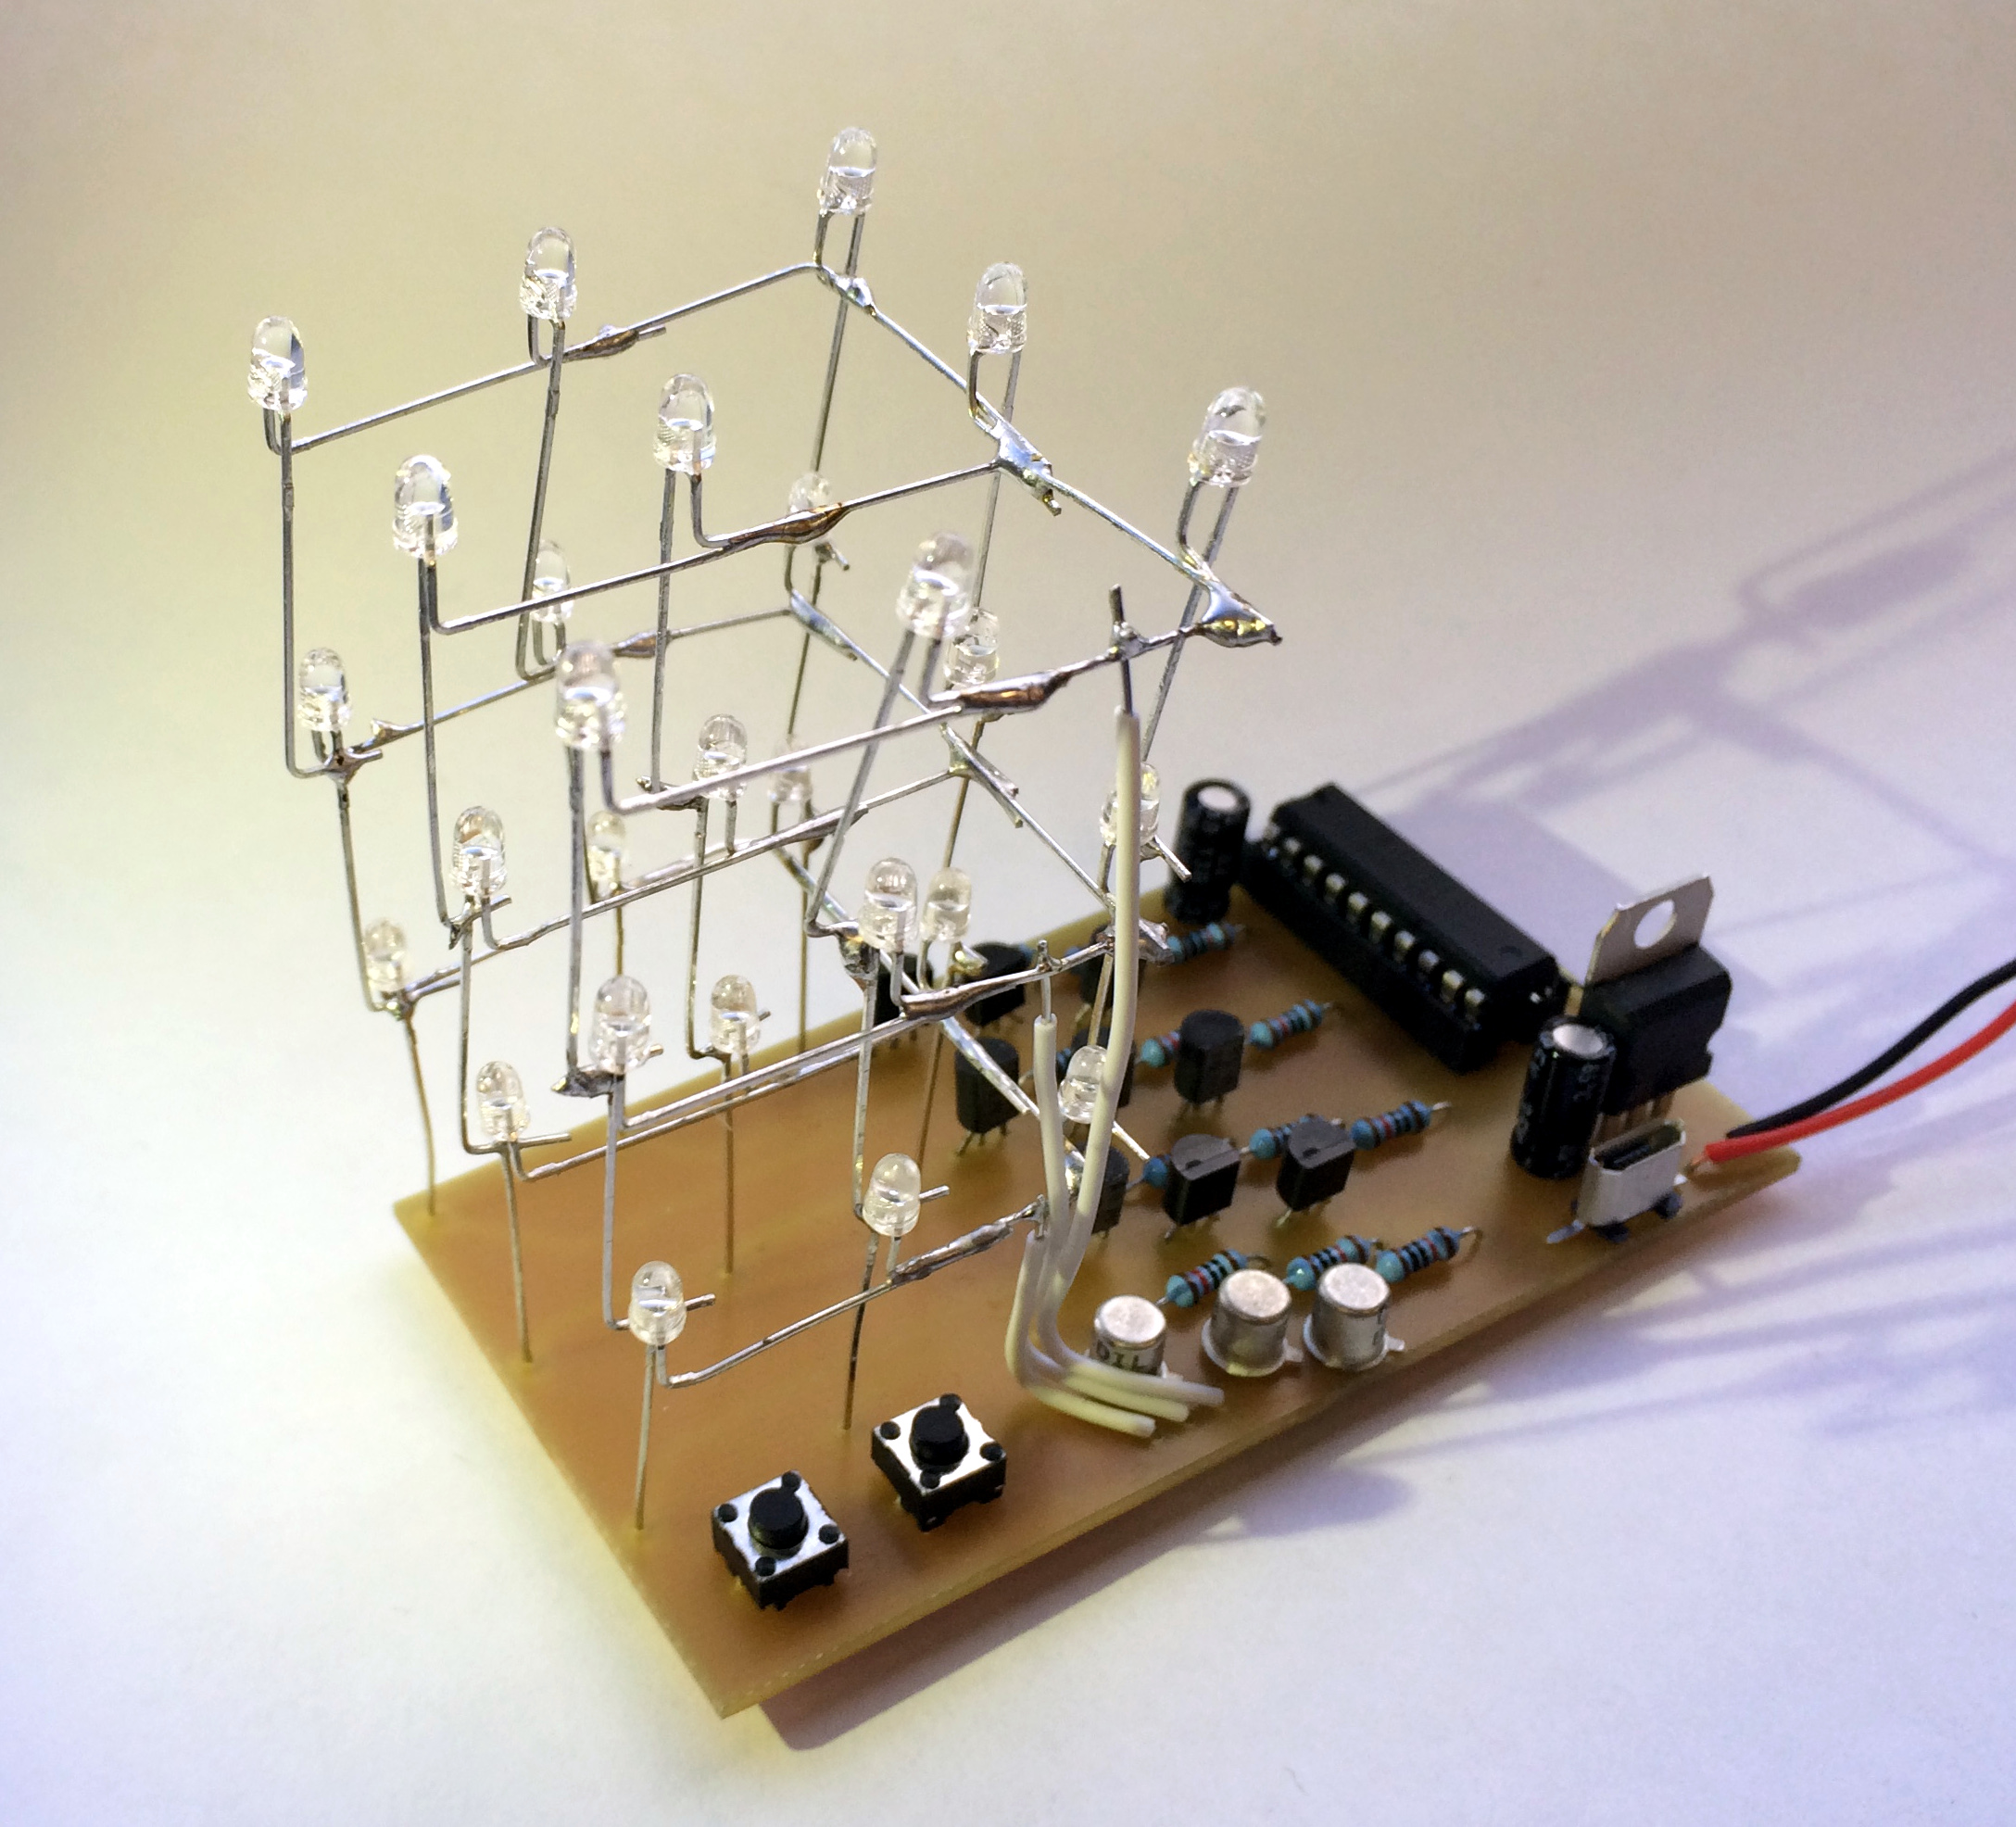
\includegraphics[width=0.8\textwidth]{photo_of_cube.JPG}
}



\section{Component list}
\centerline{
\begin{tabular}{@{}lll@{}}
\toprule
\textbf{Component} & \textbf{Spec}             & \textbf{Quantity} \\ \midrule
Transistor         & BC327                     & 9                 \\
Transistor         & BC108                     & 3                 \\
Resistor           & 10K 250mW                 & 12                \\
DIL Socket         & 20 pin                    & 1                 \\
MCU                & MSP430G2553*              & 1                 \\
Switches           & SPST tactile              & 2                 \\
Power Connector    & MicroUSB, through-hole    & 1                 \\
Resistor           & 47K, 250mW                & 1                 \\
LED                & Red, superbright, 3mm     & 27                \\
Capacitor          & 10$\mu$F, Electrolytic & 2                 \\
Power Regulator    & LM317                     & 1                 \\
Resistor           & 240R, 250mW               & 1                 \\
Resistor           & 430R, 250mW               & 1                 \\ \bottomrule
\end{tabular}
}

*Any 20 pin MSP430G2xxx microcontroller can be used. The 2553 was chosen 
because it has the most memory, so can store the most animation. %TODO has this changed?

\section{Component placement:}
The below figure shows the component placement that is not obvious from
the board's silkscreen.

\centerline{
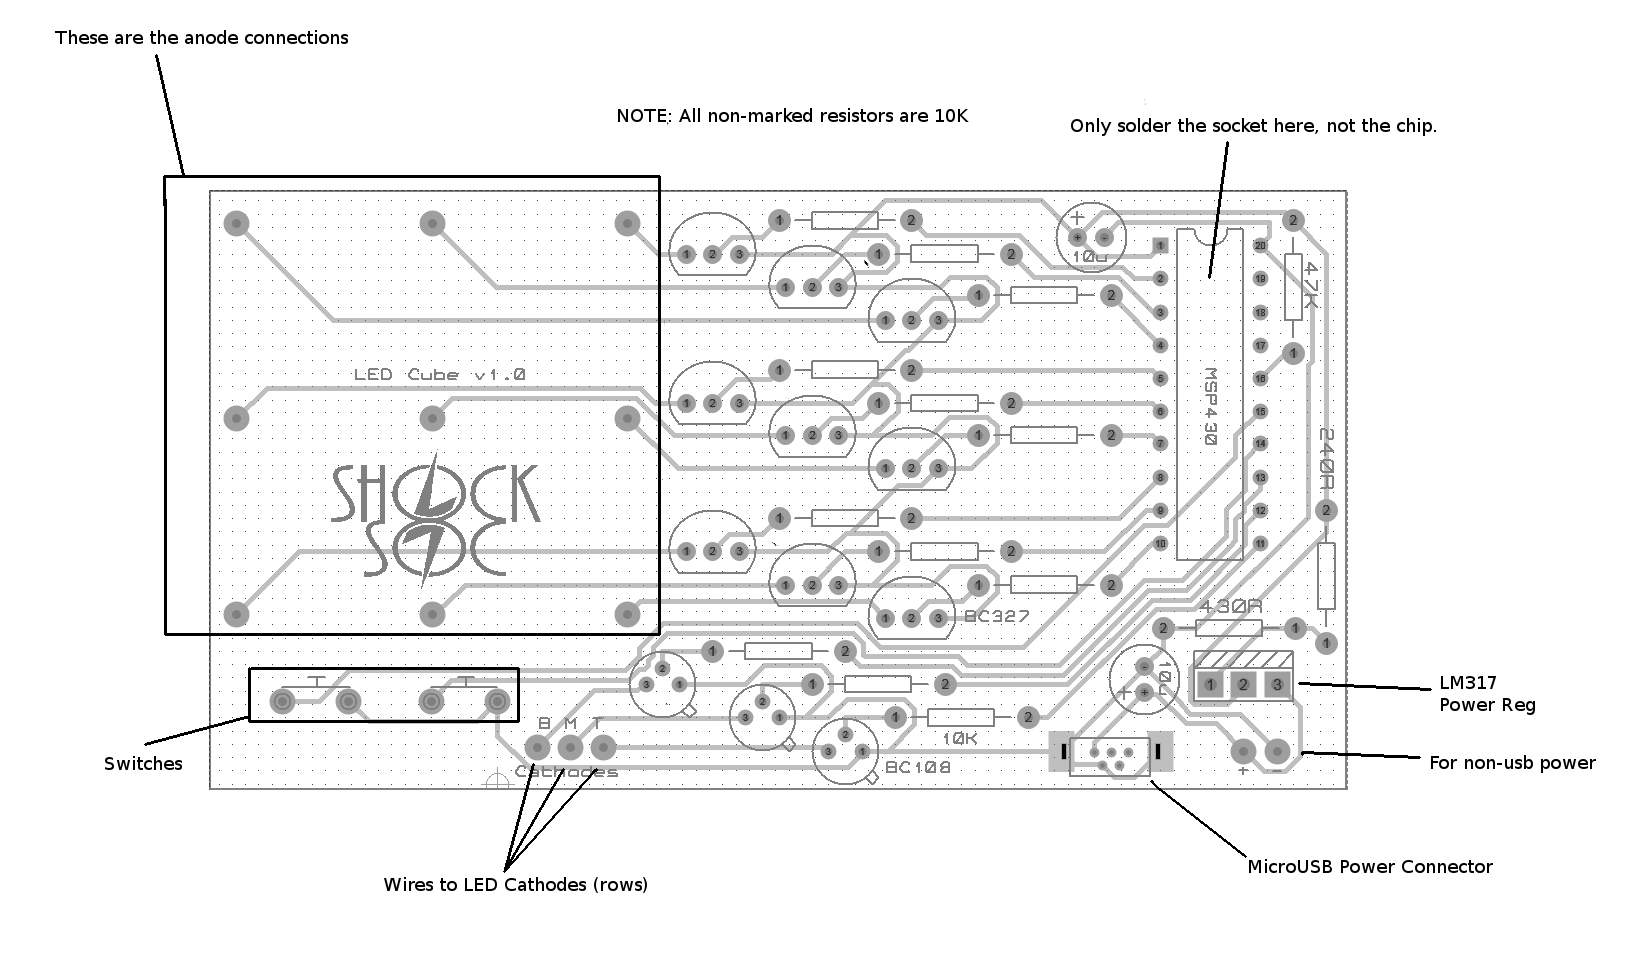
\includegraphics[angle=90, width=0.8\textwidth]{board_layout.png}
}

Some explanation is required: 
\begin{itemize}
\item All non-marked resistors are of 10K$\Omega$ value

\item The transistors should only fit into the correct holes, but the
bottom three are the BC108 transistors, and the top 9 are BC327.

\item See next section for soldering the LEDs
\end{itemize}

\section{LED Soldering}
The LEDS have two leads, the cathode (negative, shorter lead) and the 
anode (positive, longer lead). Each of the 9 columns of LEDs have their
anodes connected together, and the bottom anode of each column should be
soldered into the PCB (in the holes marked anodes on the previous 
diagram). Then, each row has its 9 LEDs' cathodes connected together. 
These are connected by wire the the three holes labelled cathodes. B, M, 
T denotes the bottom, middle and top rows.

In order to actually solder the LEDs, a jig has been provided, picured 
below. %TODO: Add photo


The three holes are to place the ends of the LEDs in to space them 
correctly and hold them in place whilst soldering. The end bit is for 
bending the leads consistently. 

The process is as such
\begin{enumerate}
\item Bend the LED leads, making sure the anode is bent near the end of
the lead and the cathode (shorter lead) is bent close to the LED. Follow
the markings on the jig.

\item Solder three LEDs' cathodes together (repeat 9 times)

\item Solder 3 sets of the LEDs' anodes together. You should now have 3 
three-by-three grids of LEDs. 

\item You should now have 3 three-by-three grids of LEDs. These should 
be soldered into the PCB (put the anodes in the relevant holes).

\item Connect the remaining cathodes together on each row.

\item Add wires between the rows on the cathode and the holes on the 
PCB.

\end{enumerate}

I've tried to do some diagrams of this, but a clear LED with a clear
acrylic jig is really hard to photograph. On the otherhand, 27 LEDs in
a 3D cube arrangement is really hard to draw, so there's a mix. 

\centerline{
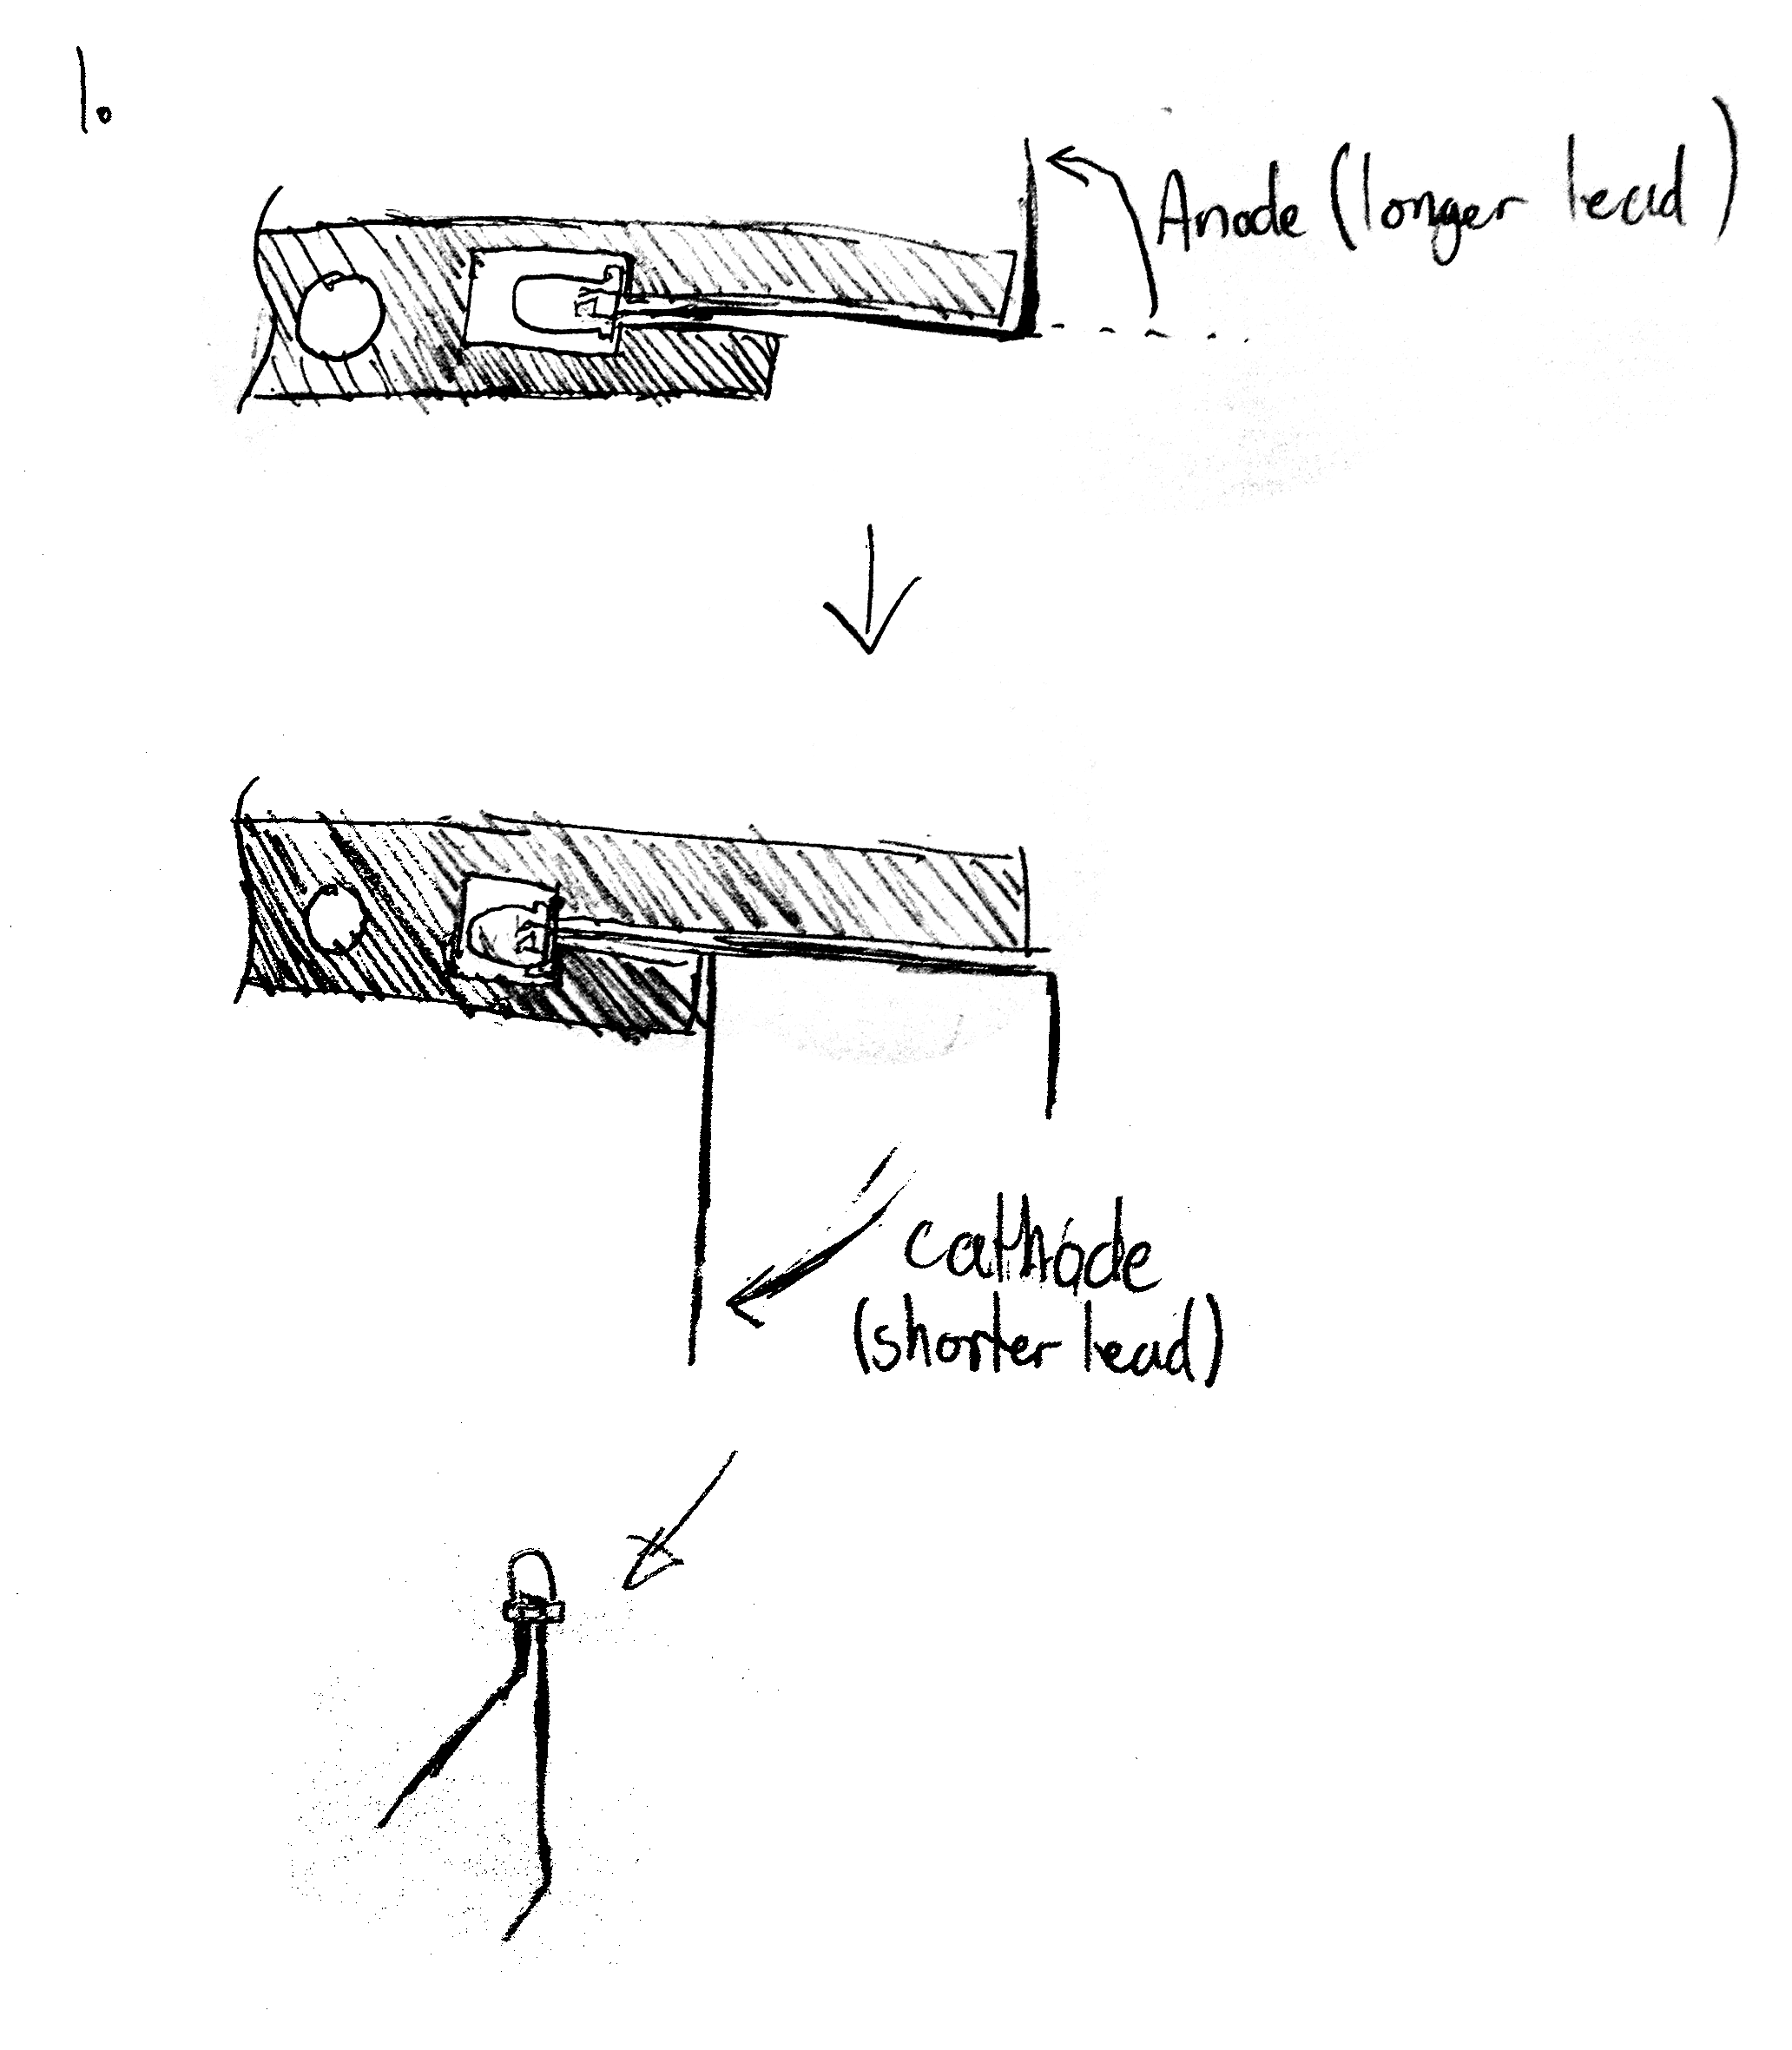
\includegraphics[width=0.8\textwidth]{s1.png}
}

\centerline{
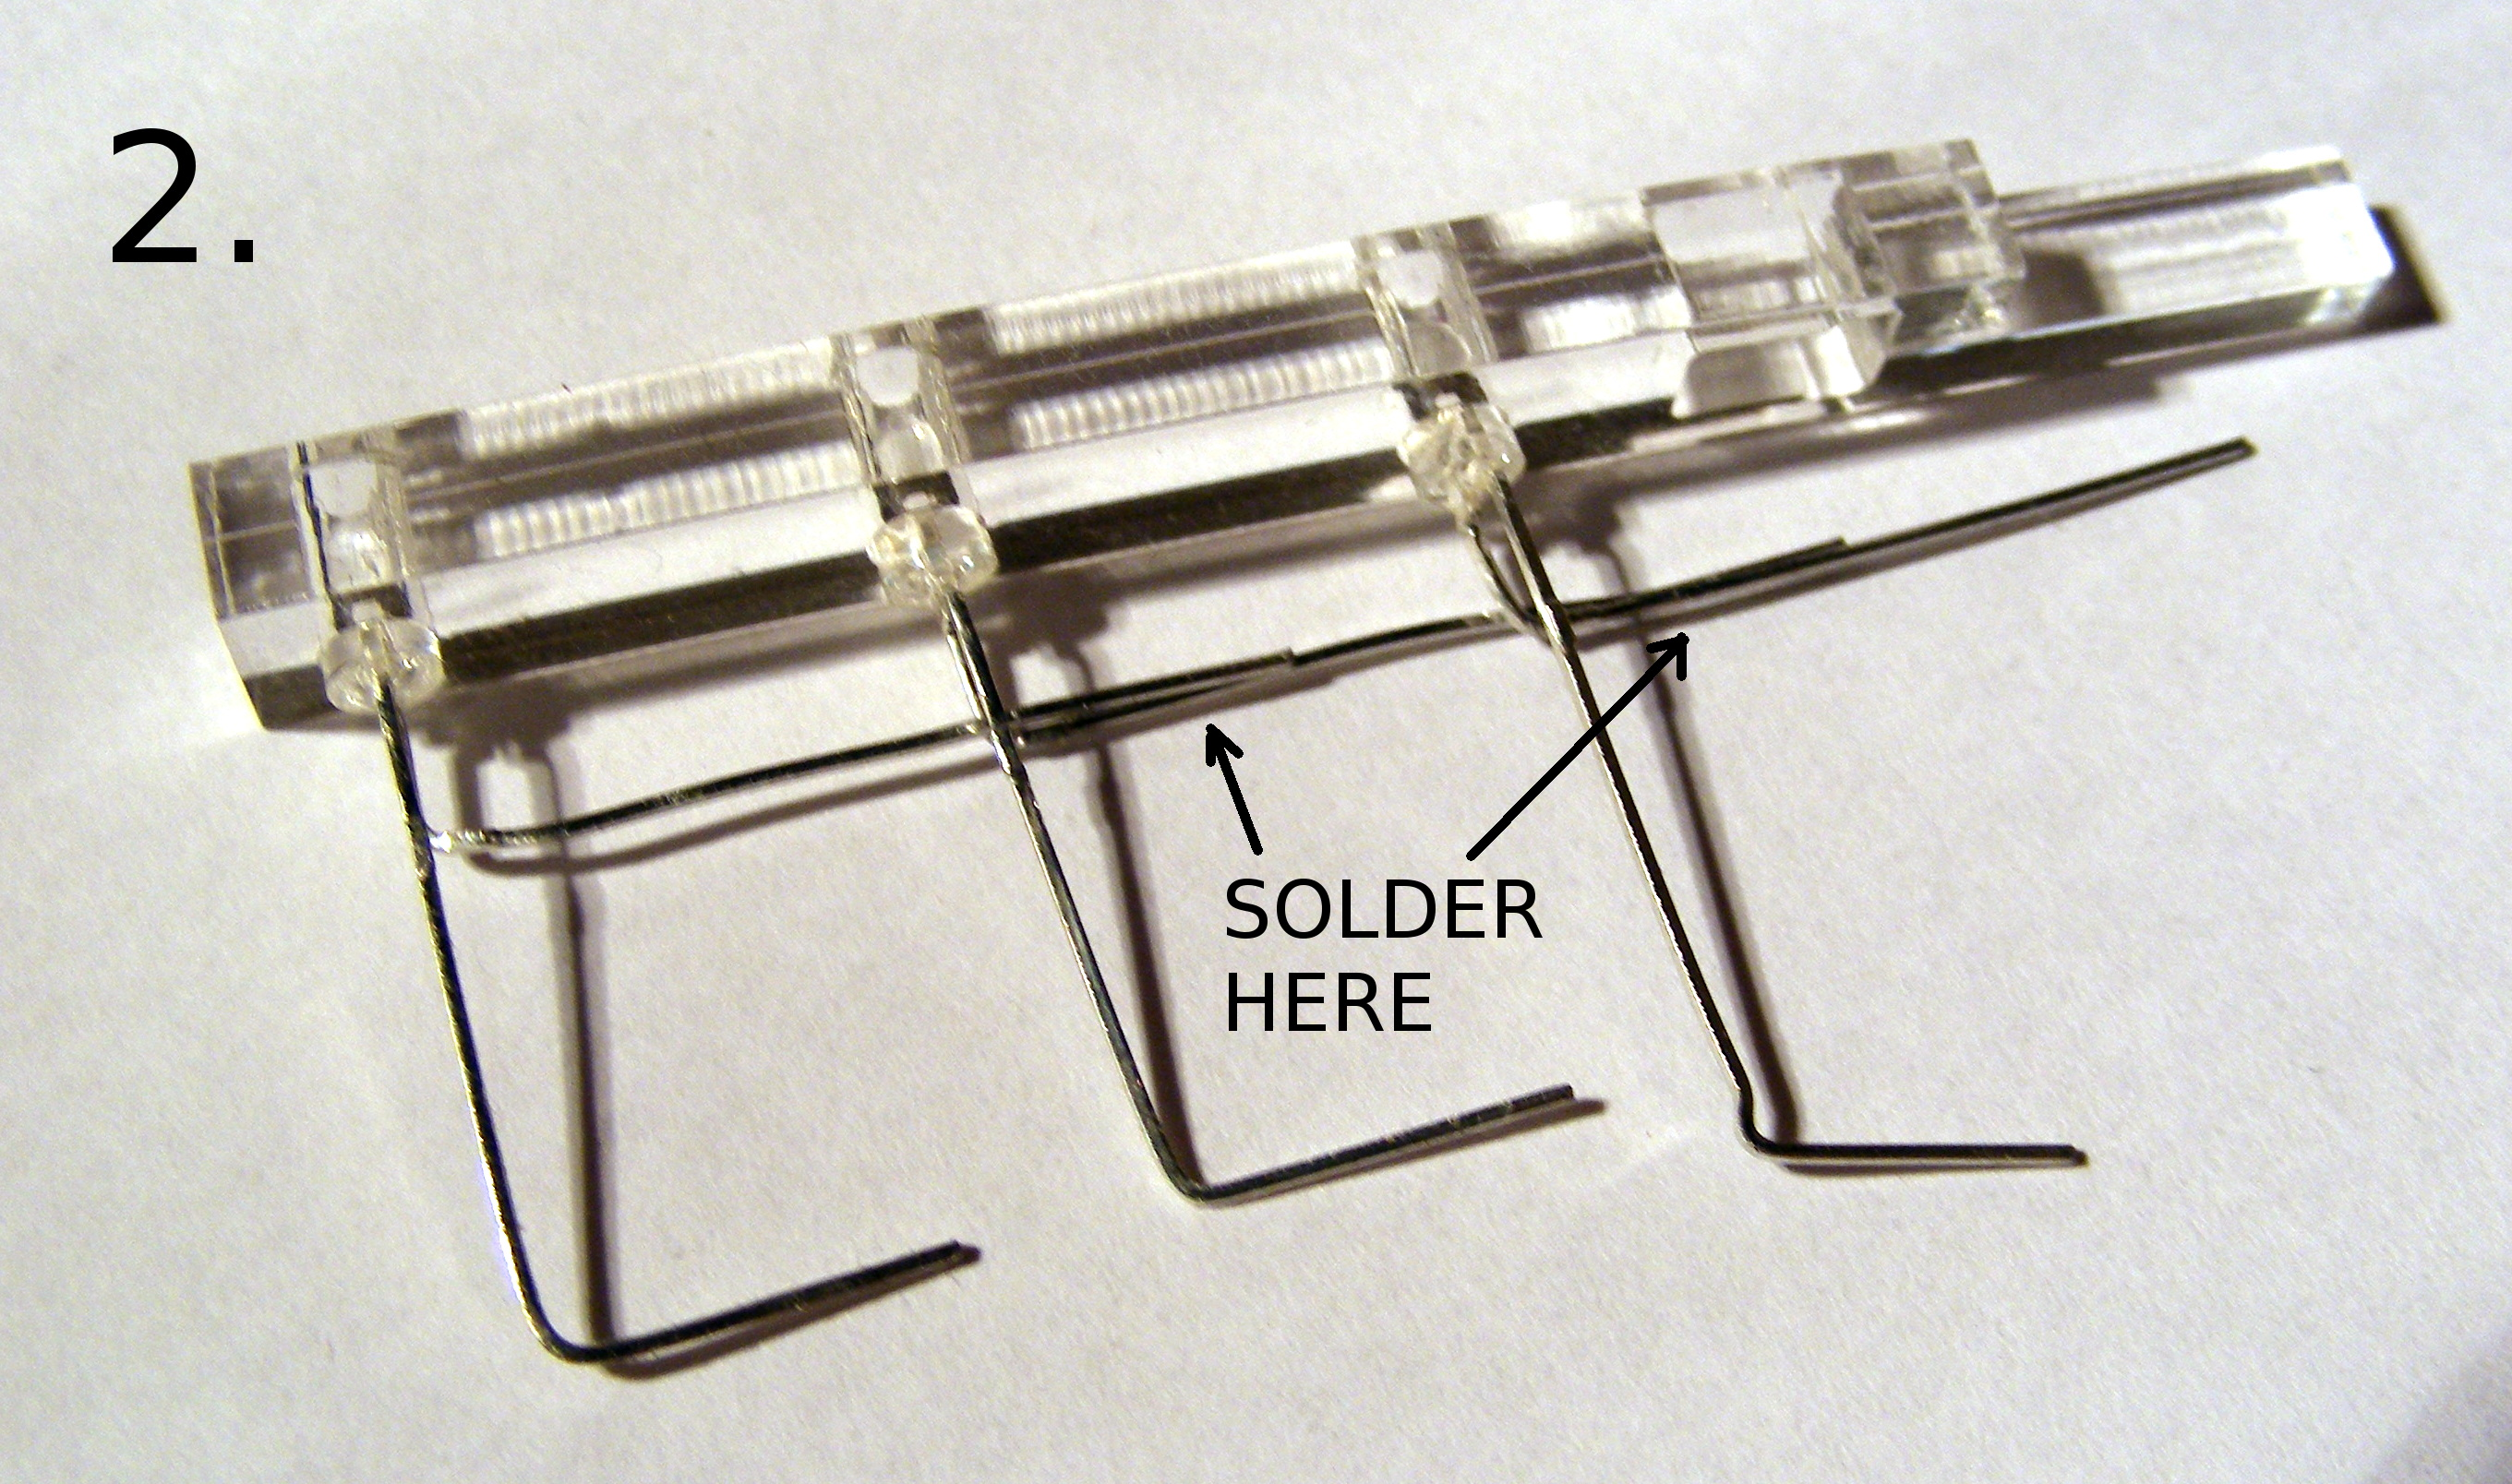
\includegraphics[width=0.6\textwidth]{s2.JPG}
}

\centerline{
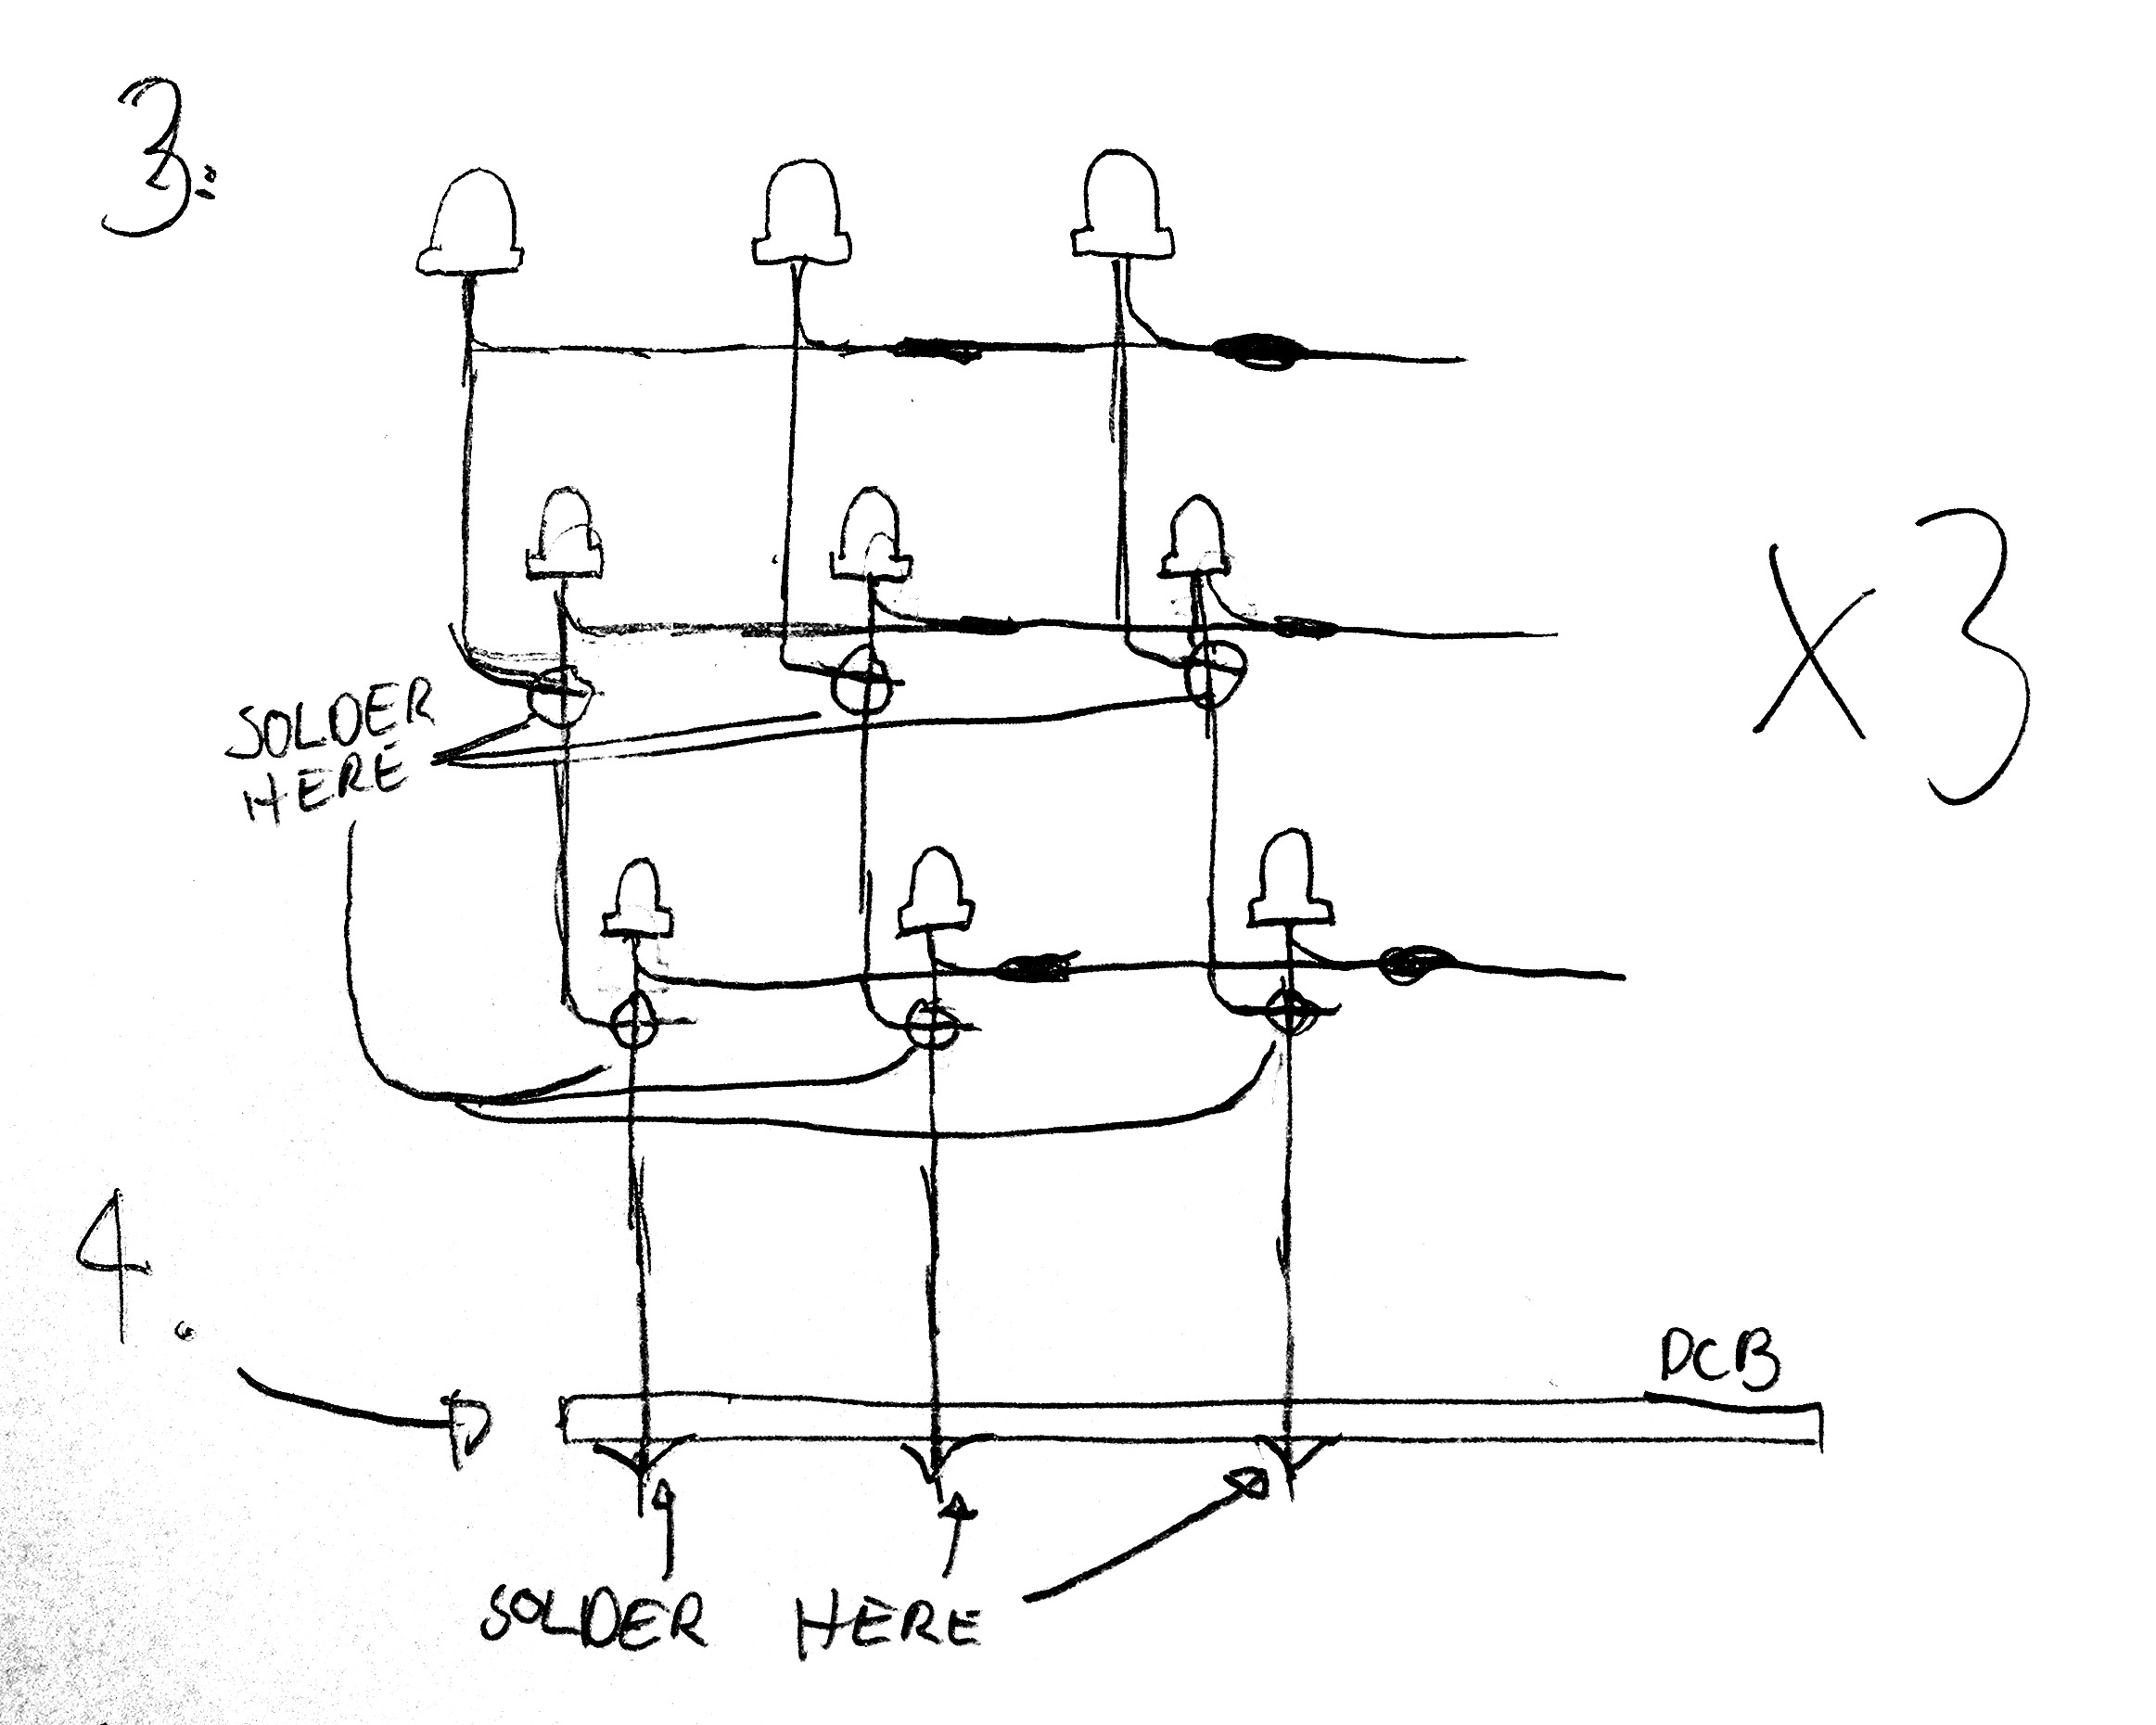
\includegraphics[width=0.8\textwidth]{s34.JPG}
}

\centerline{
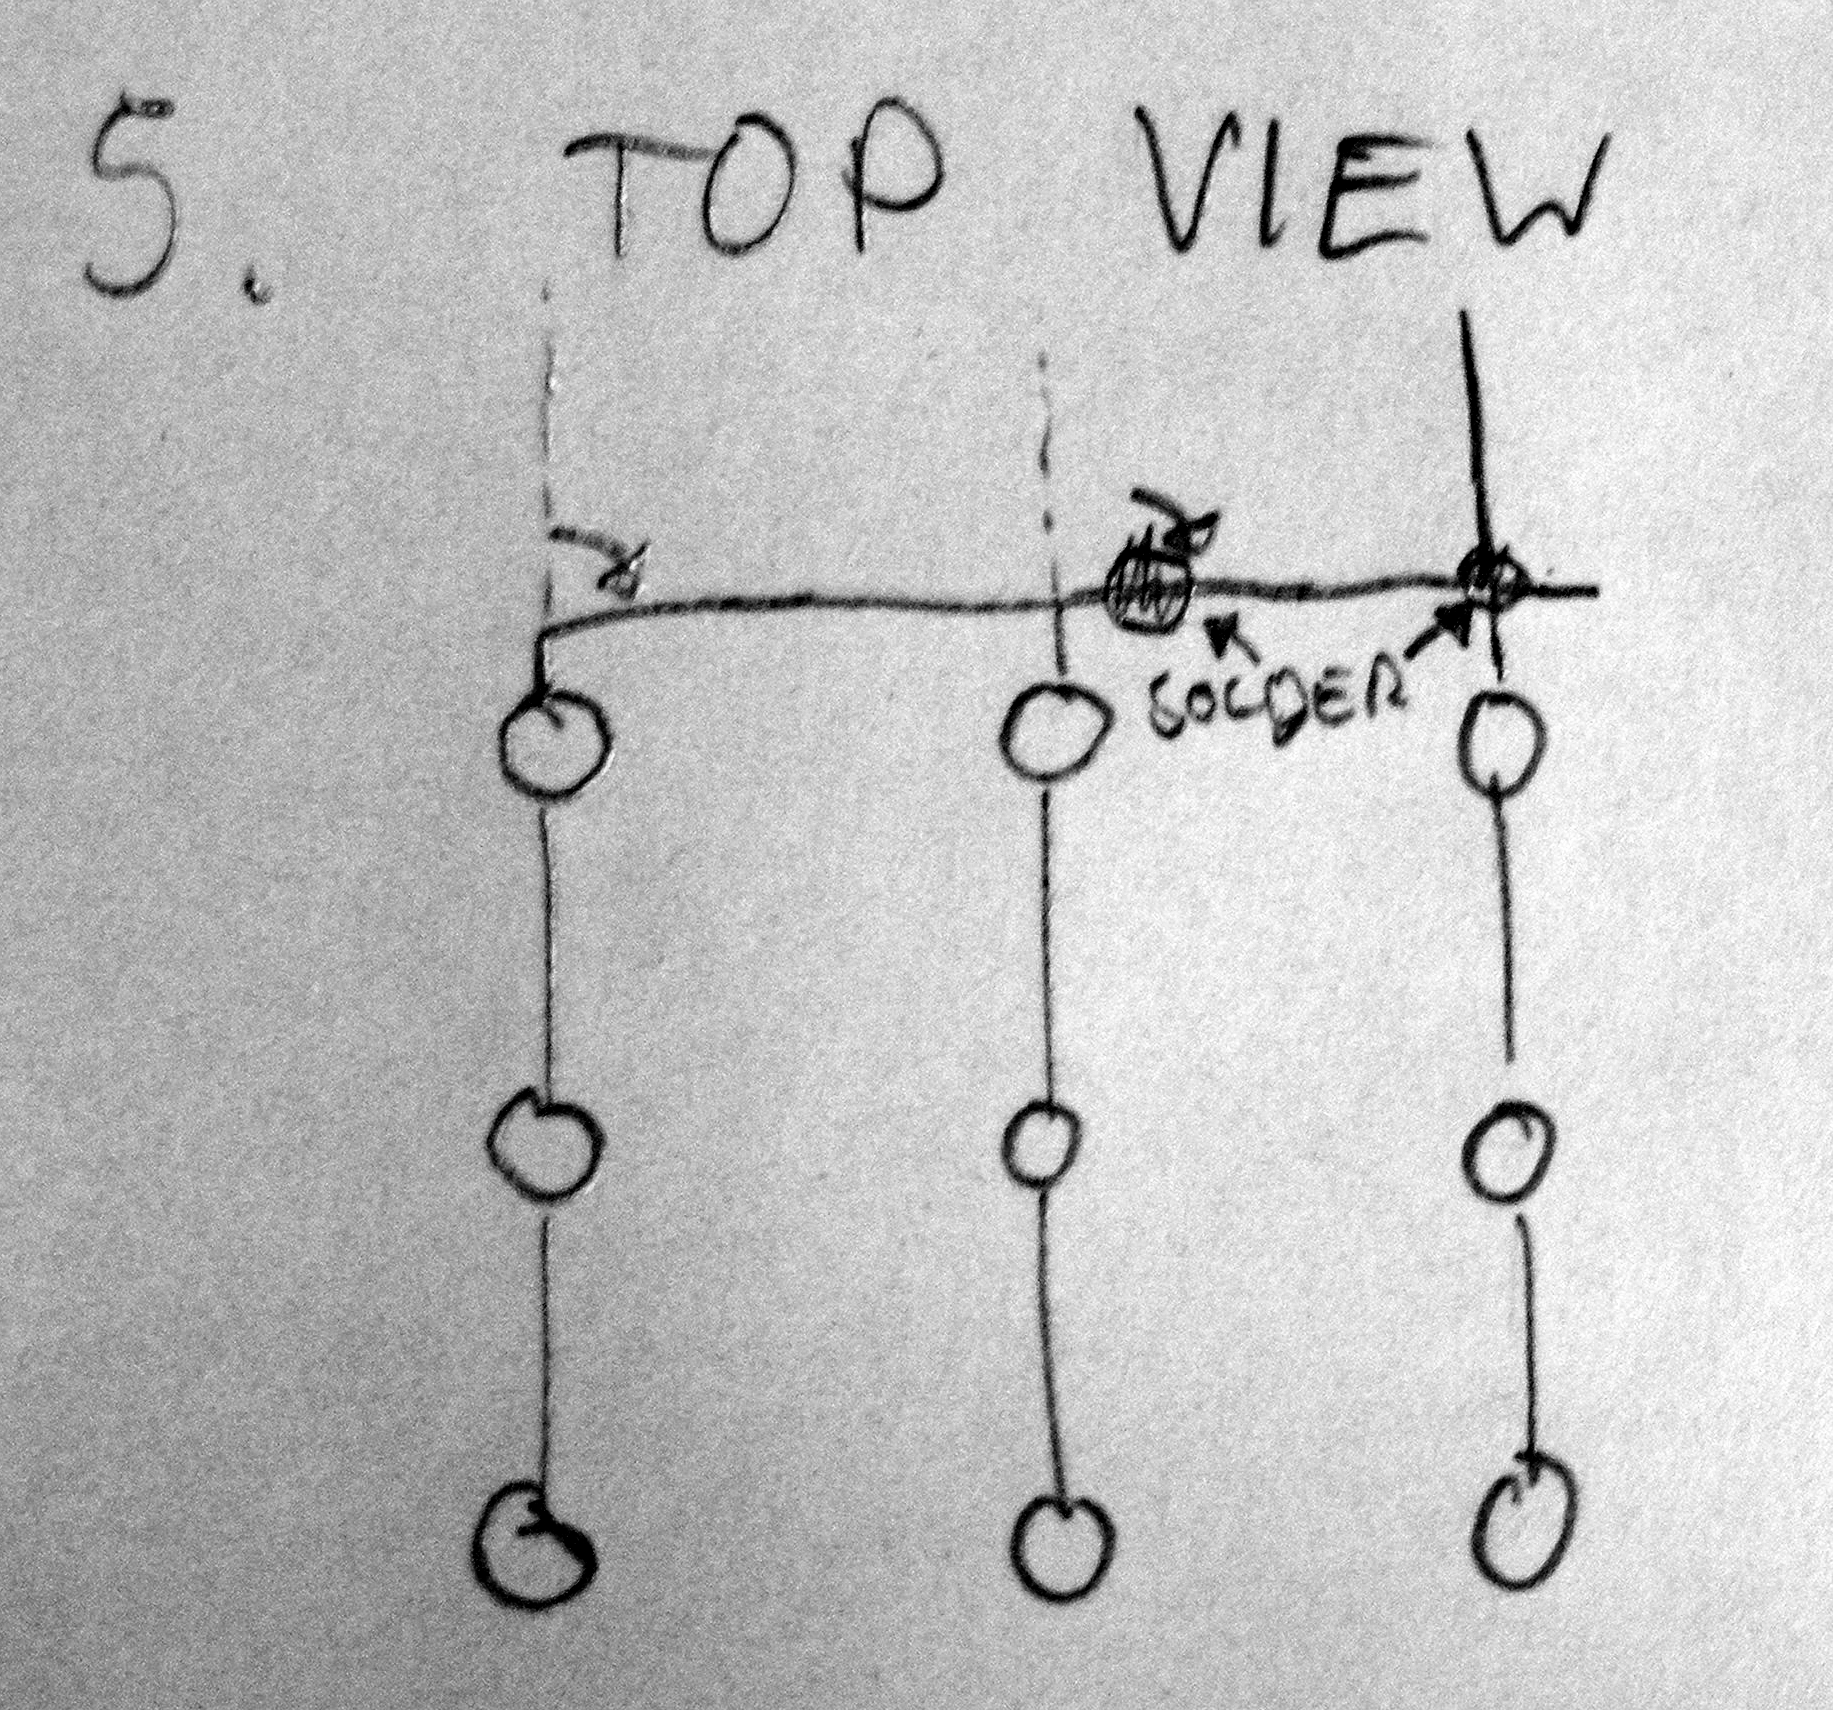
\includegraphics[width=0.5\textwidth]{s5.png}
}

\centerline{
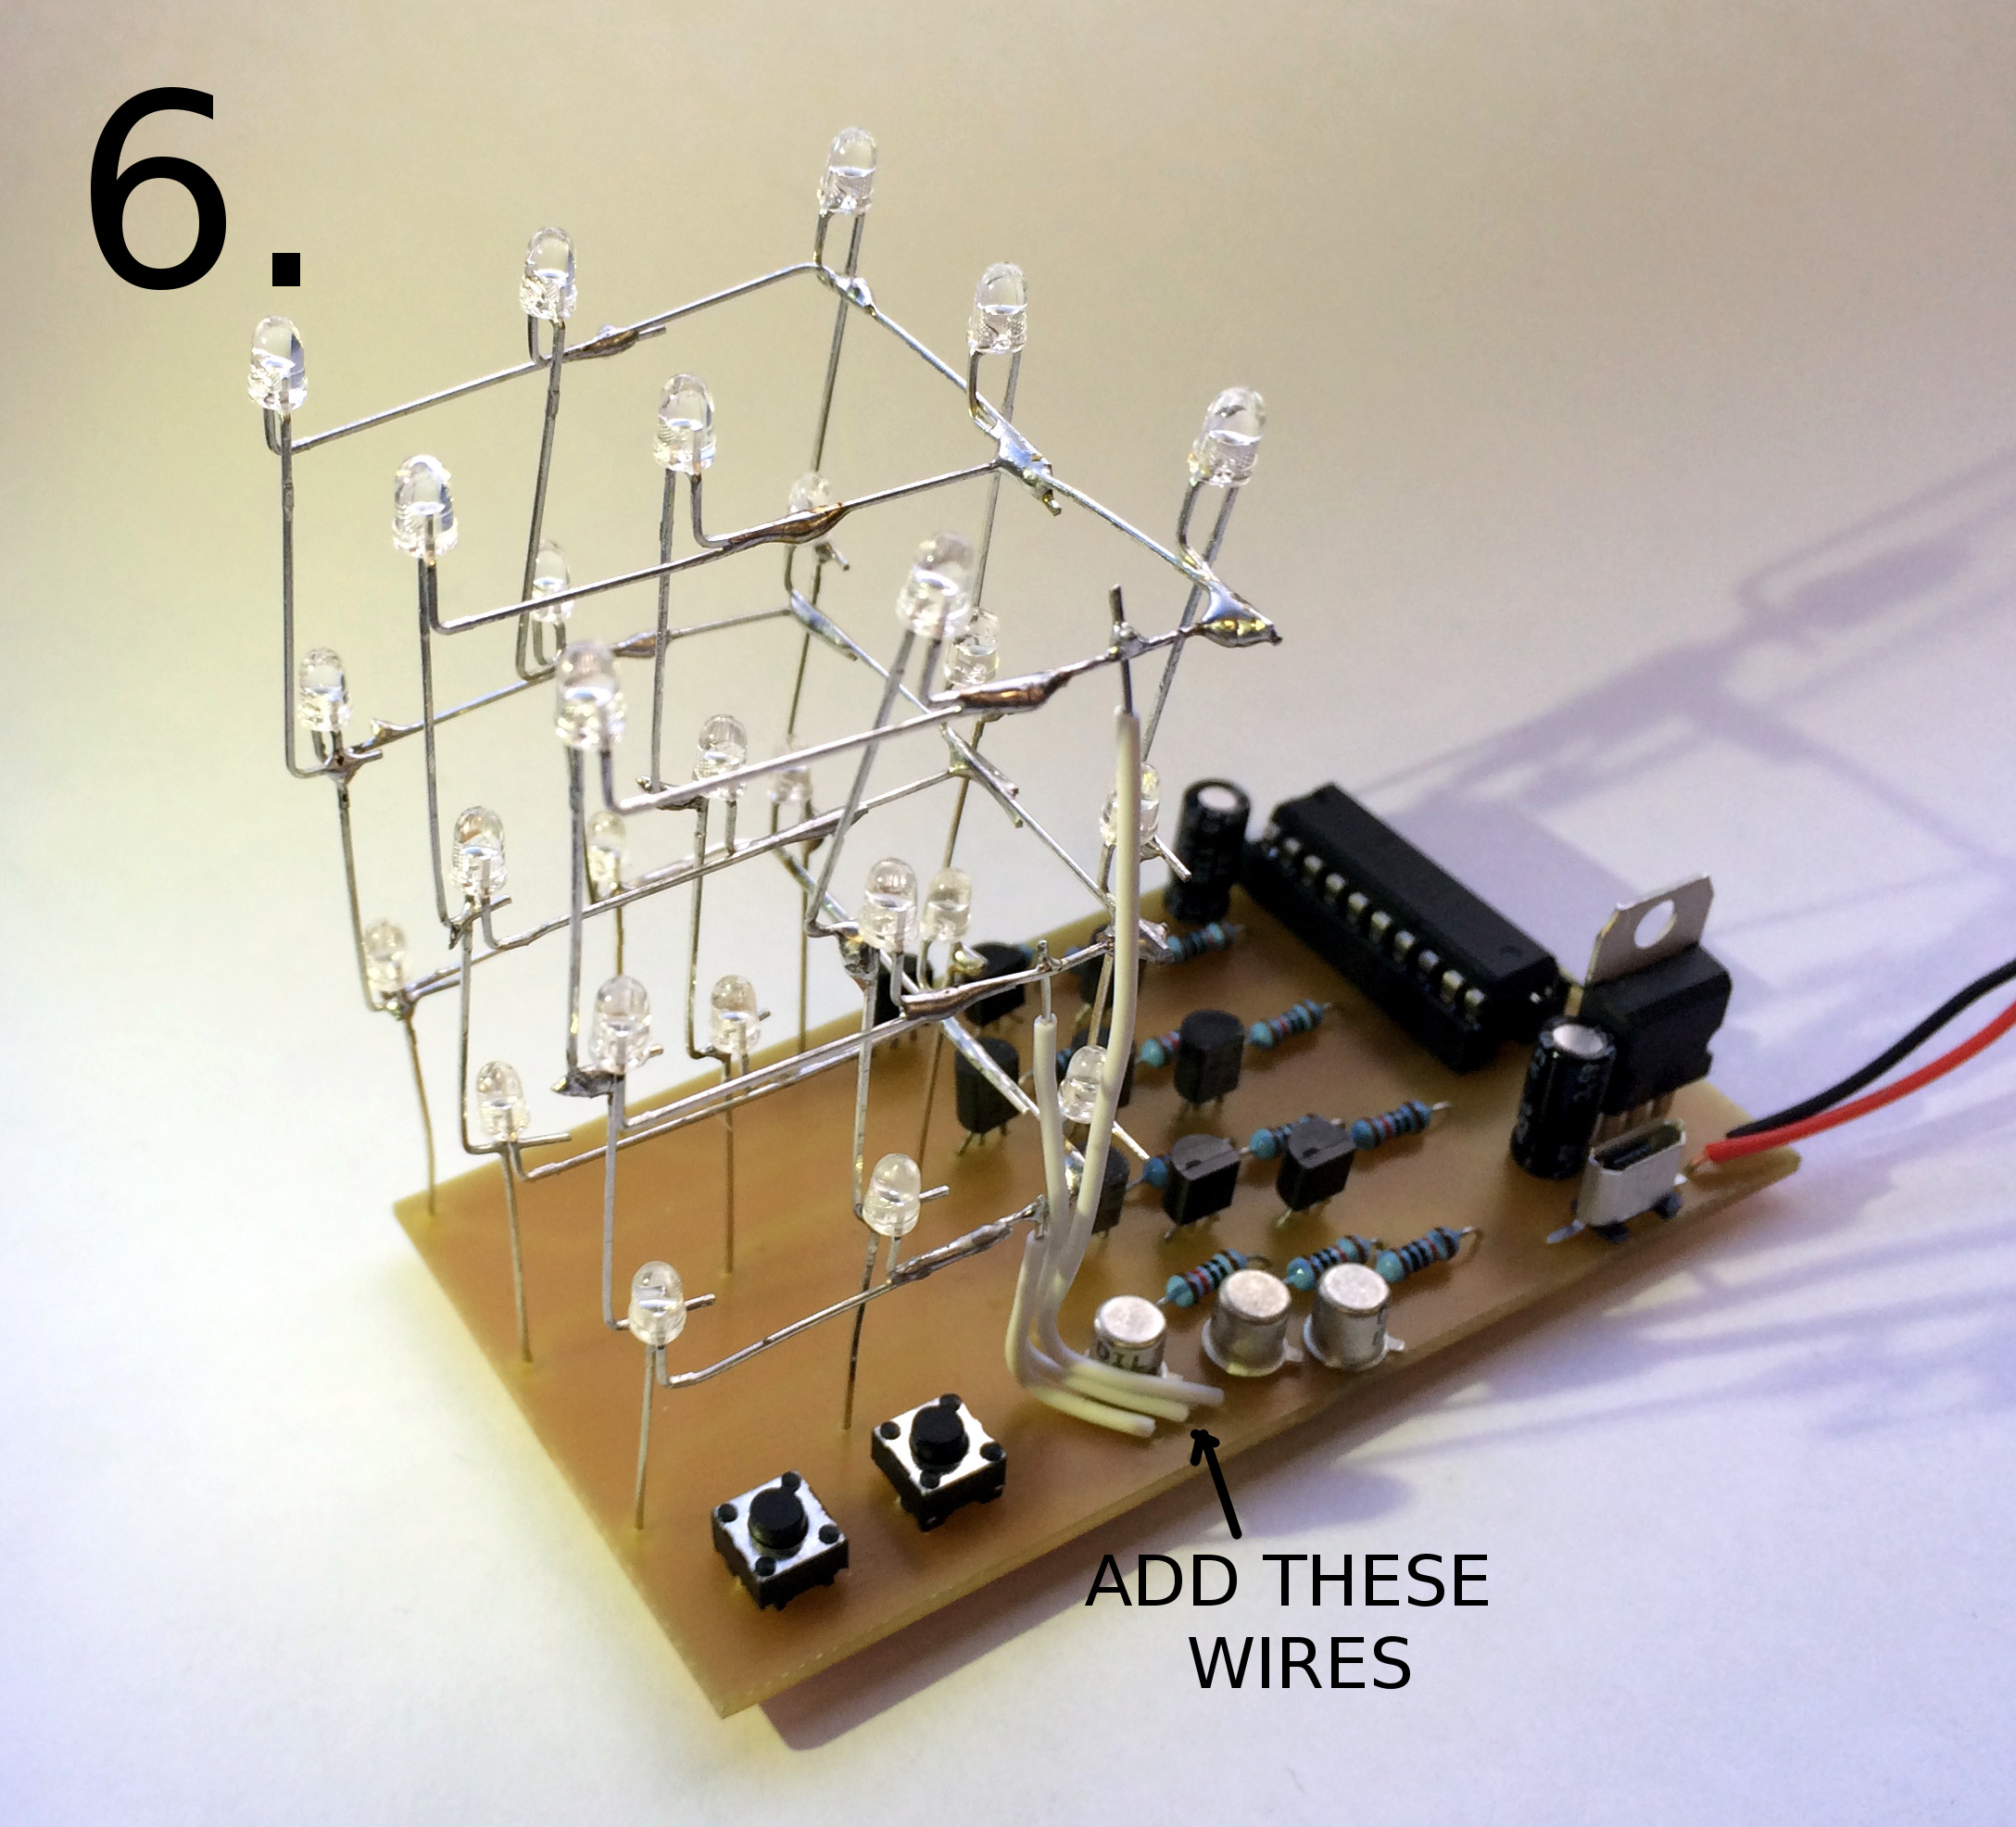
\includegraphics[width=0.6\textwidth]{s6.JPG}
}

\section{Circuit Diagram}

The below figures show the circuit diagrams for the microcontroller 
connections, power supply, and LED connections. There's also a guide to 
the coordinate system. Note that the LED is connected to two transistors. 
It's one transistor for the column that it's part of (dependant on x 
and y) and one transistor for the z column it's part of. Each transistor
is connected to more than one LED, so for example Q$_{A1,2}$ is 
connected to LED$_{1,2,0}$, LED$_{1,2,1}$, and LED$_{1,2,2}$.

\centerline{
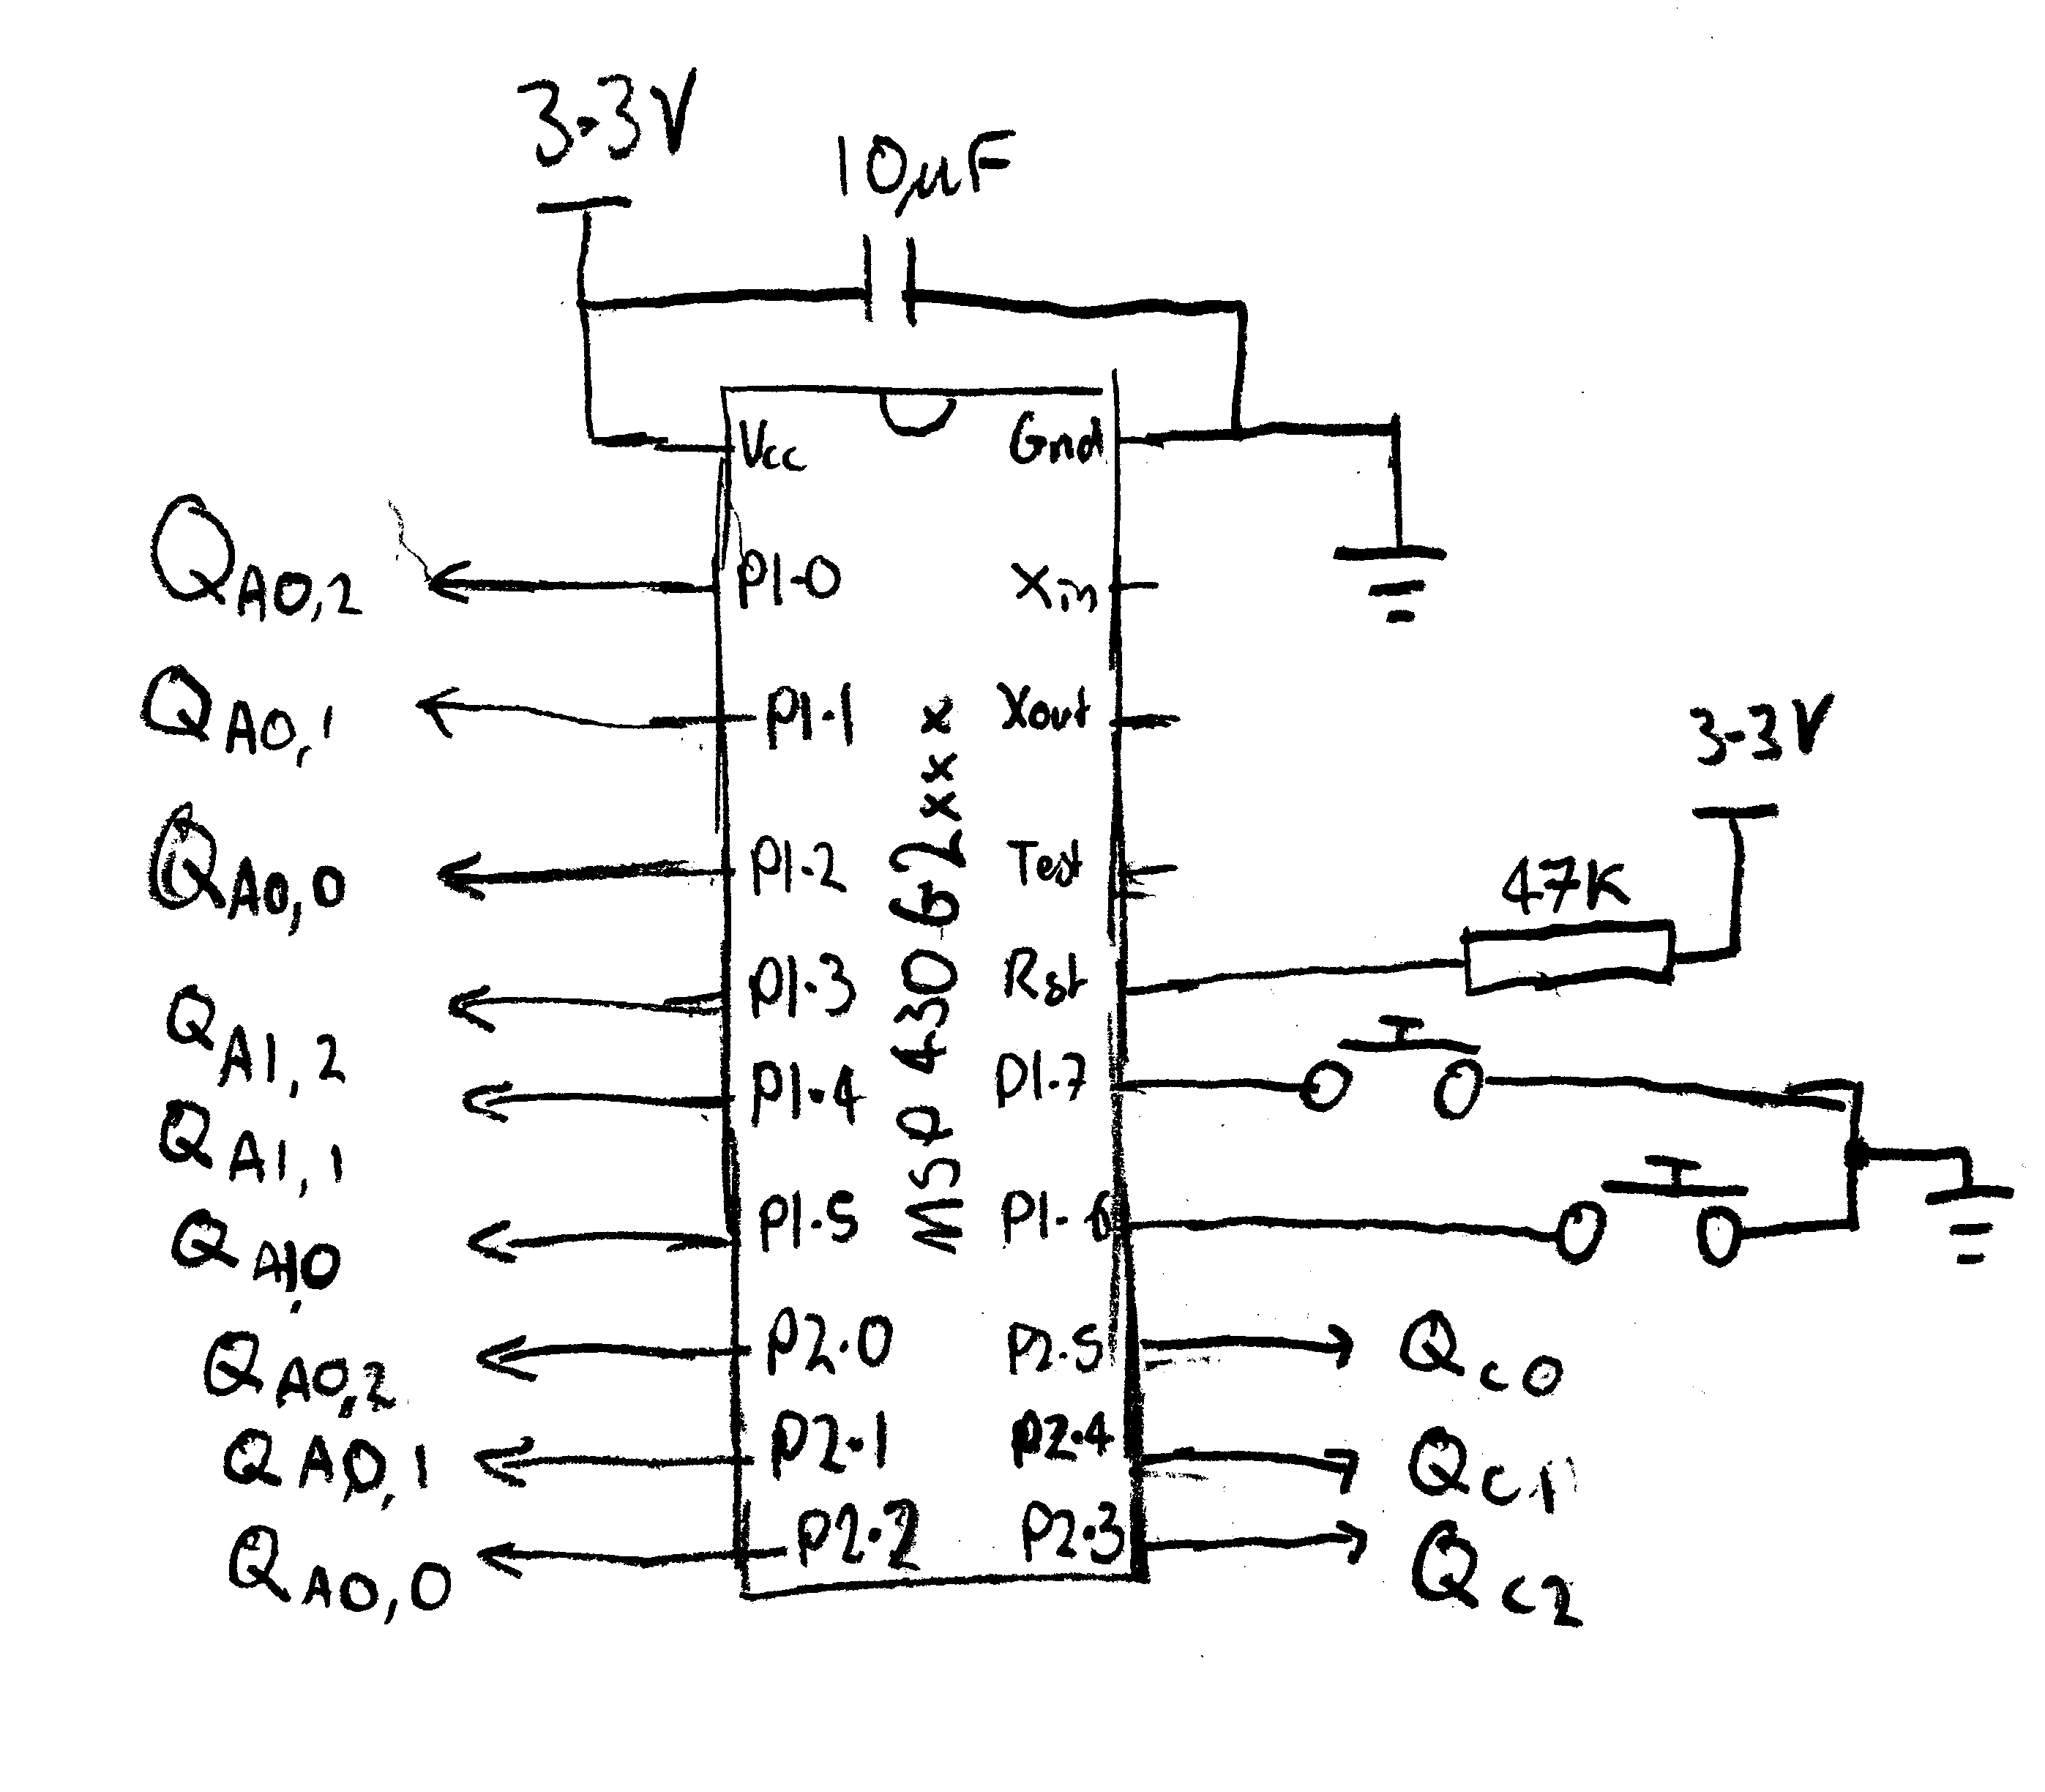
\includegraphics[width=0.6\textwidth]{mcu.JPG}
}

\centerline{
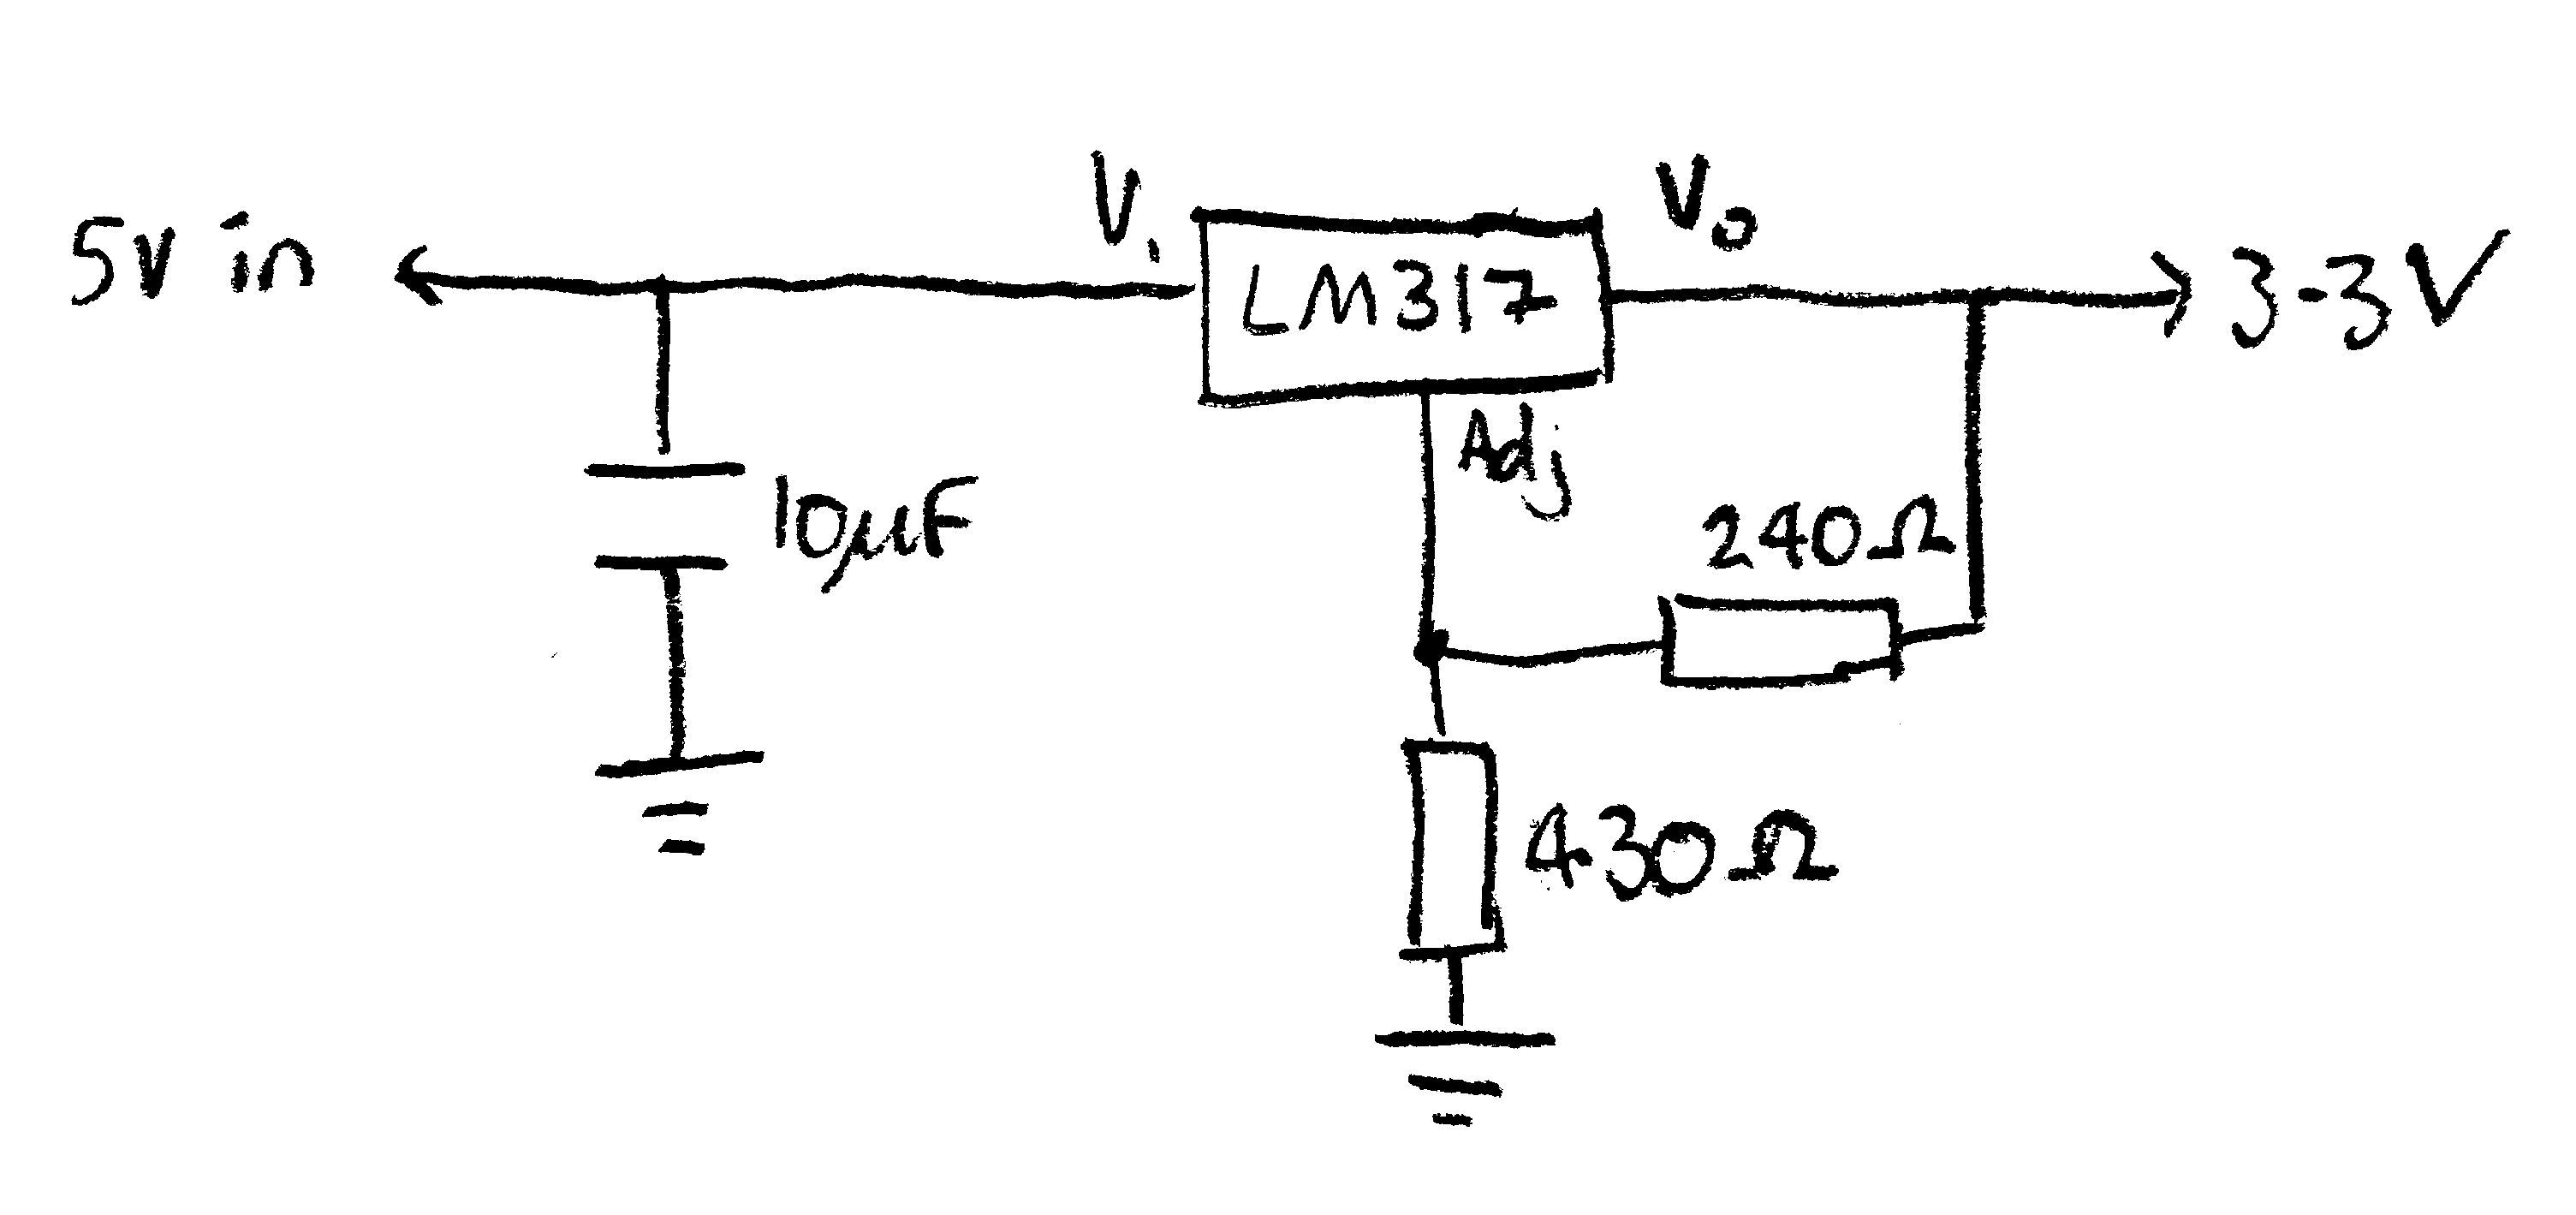
\includegraphics[width=0.8\textwidth]{pwr.JPG}
}

\centerline{
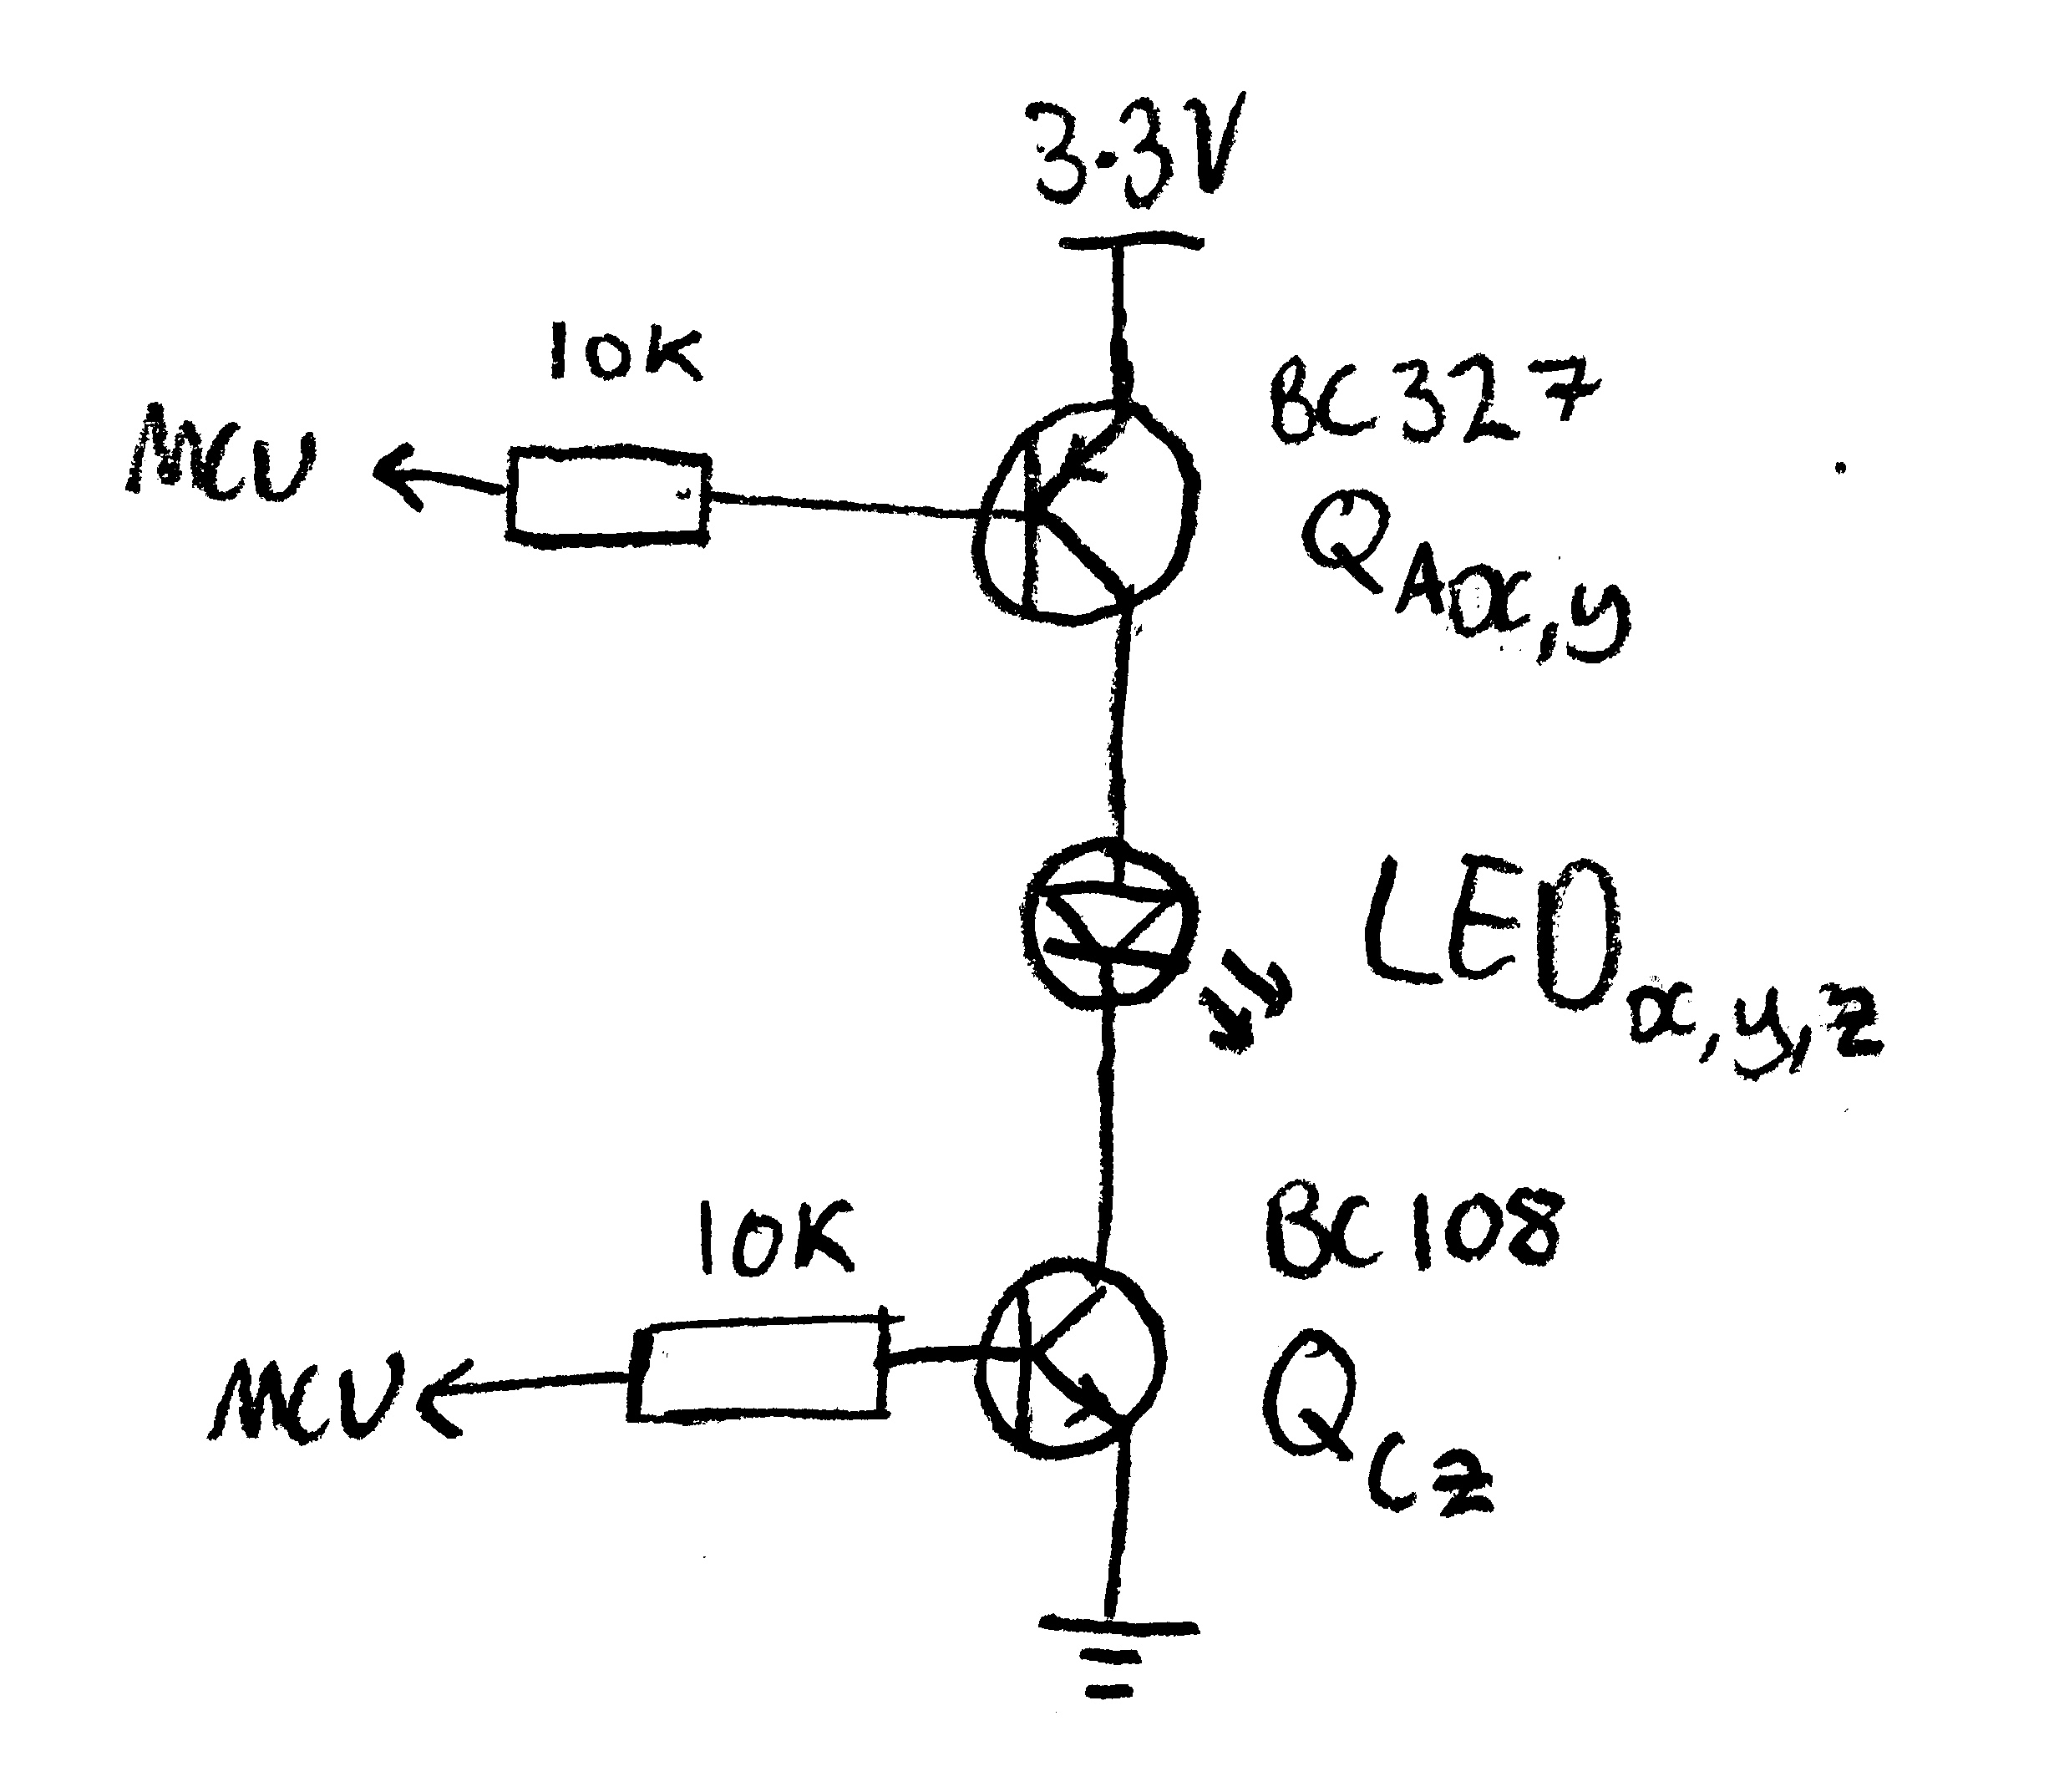
\includegraphics[width=0.6\textwidth]{led.JPG}
}

\centerline{
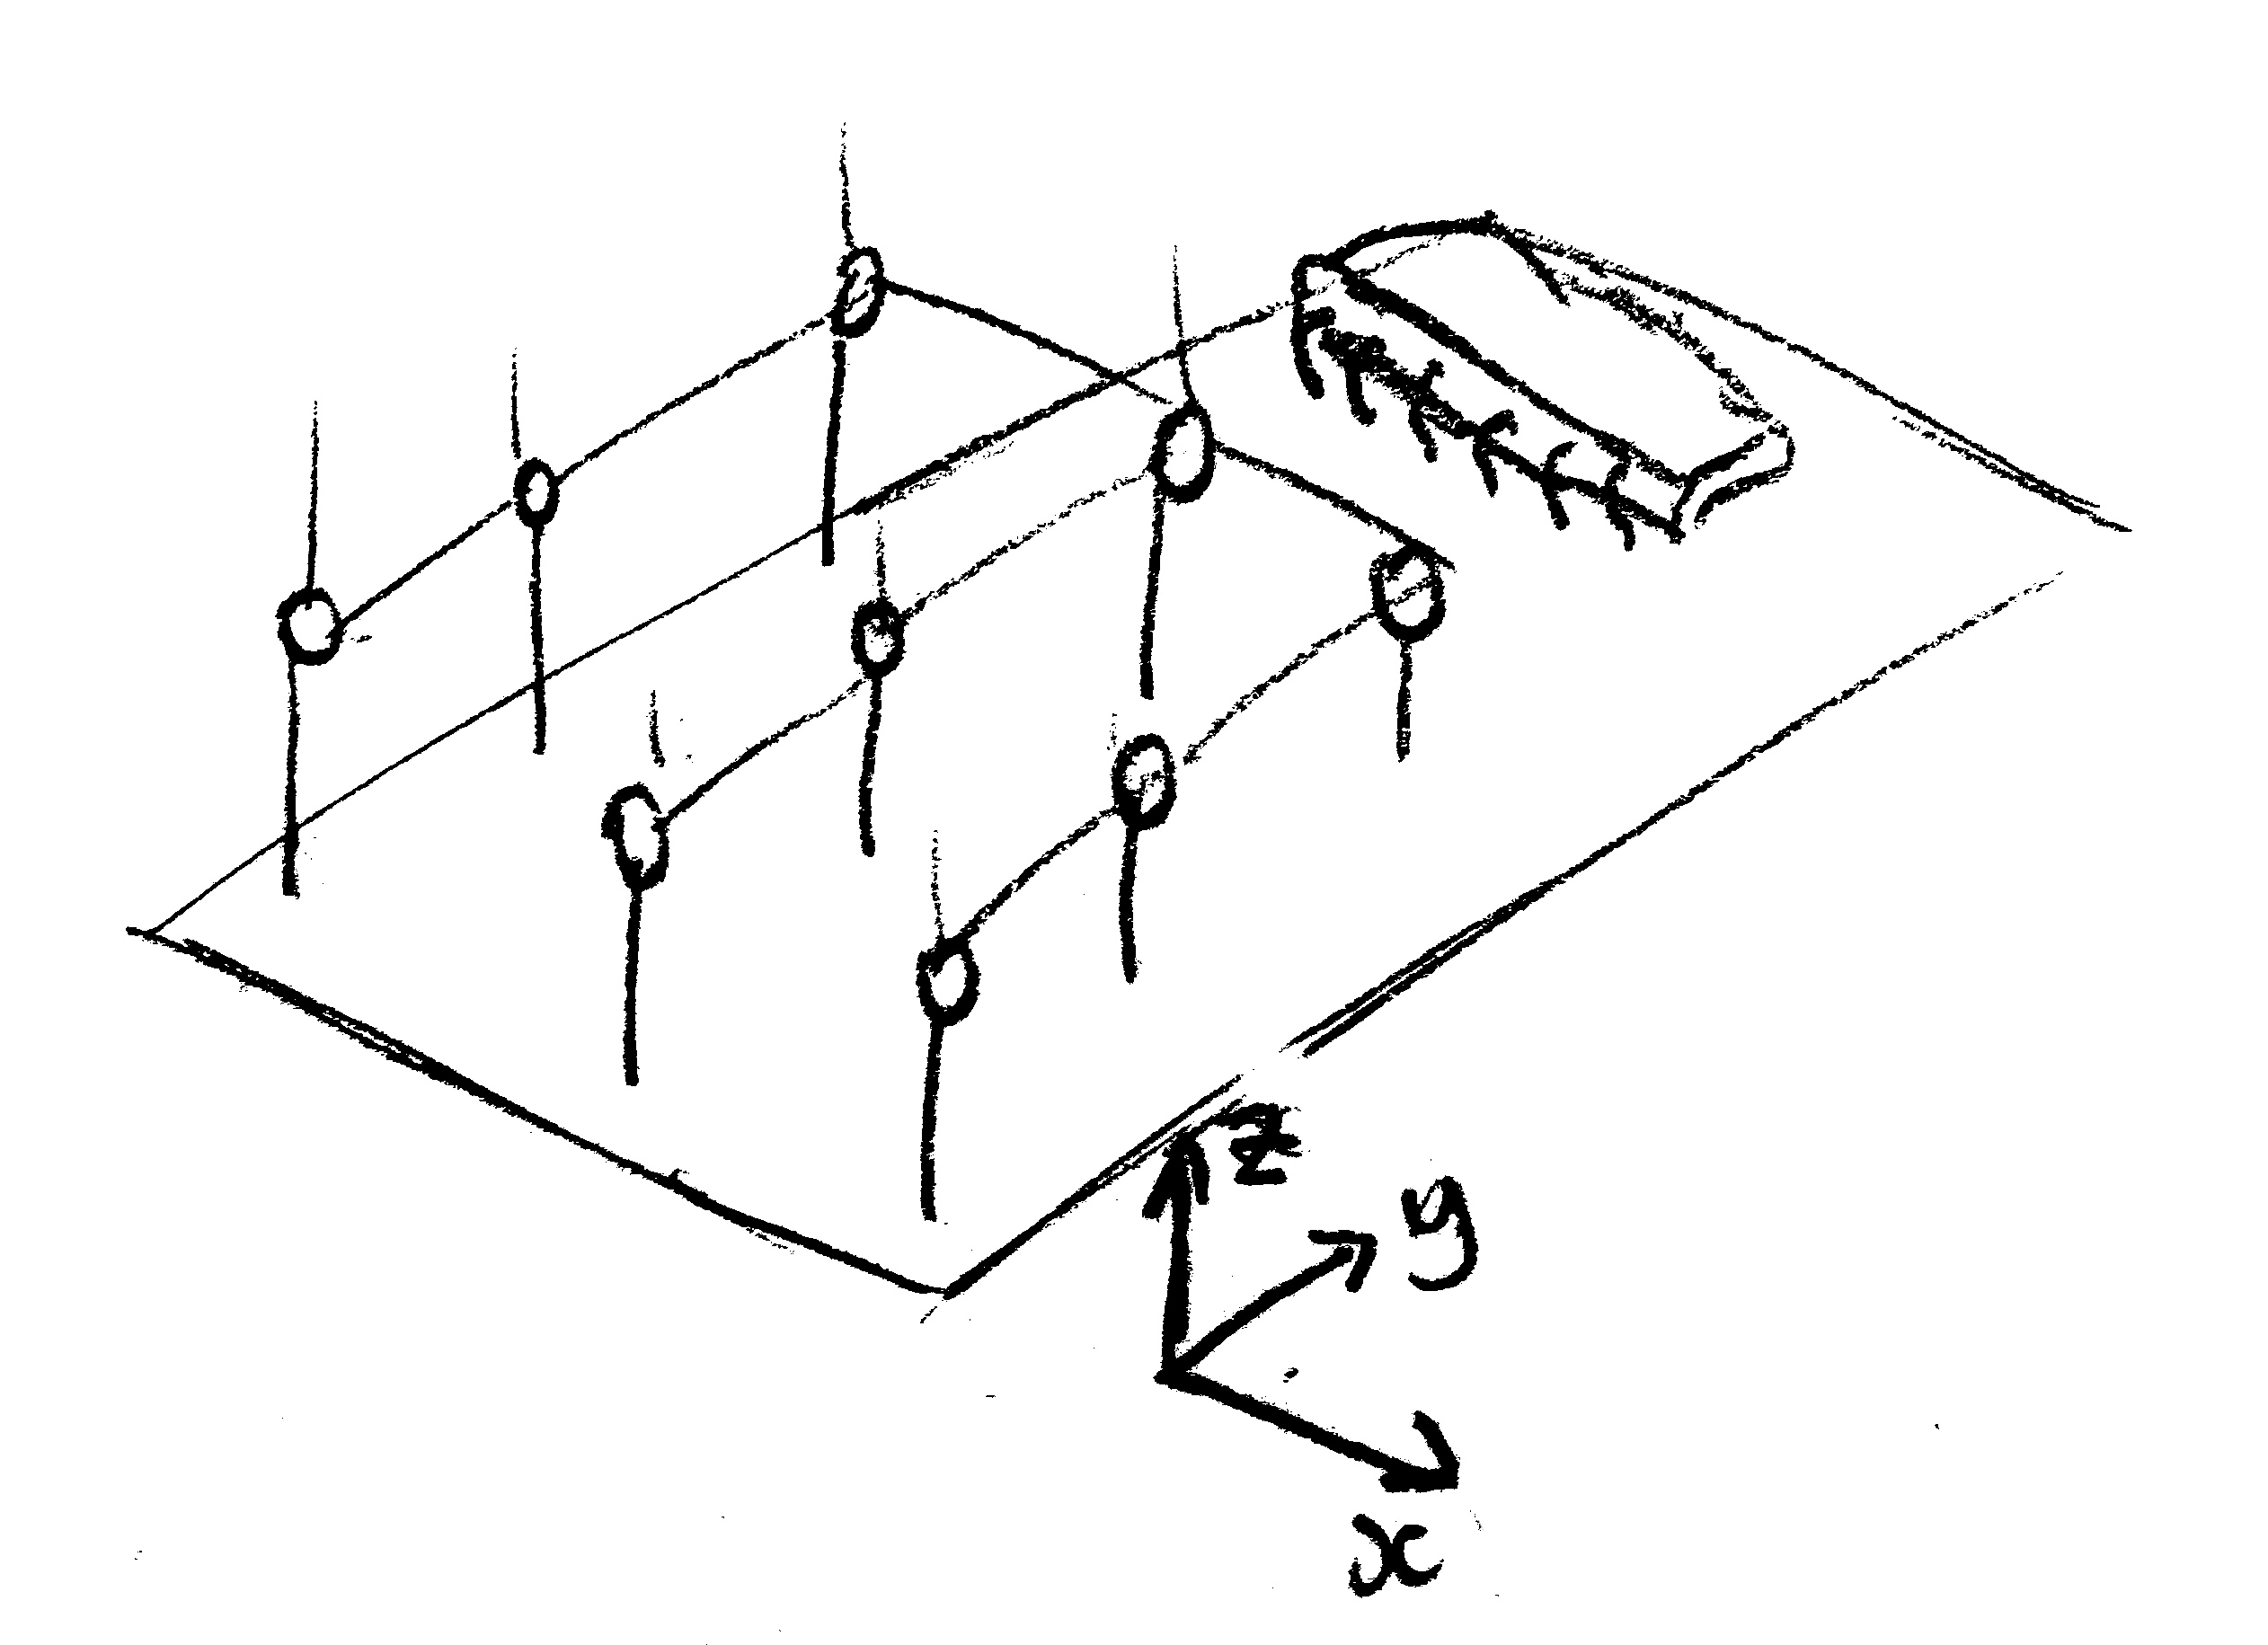
\includegraphics[width=0.6\textwidth]{coordinates.JPG}
}

				
\end{document}


